\subsubsection{ Warping }

We now explain the {\warpunit}. A warp unit generally consists of the following 5 gadgets: \prewarp,
\firstwarp, \warpbridge, \secondwarp, \postwarp. The job of these 5 gadgets is to transport the value
read by the {\cread} all the way to the digit region in the next row, so that the {\cwrite} gadgets
can write the next value in the correct locations. The {\firstwarp} and {\secondwarp} gadgets are single
tile gadgets that have north and south glues with identical labels. This allows the gadgets to continuously
assemble until stopped by earlier parts of the assembly. These single tile gadgets also have one additional glue
that will allow the next piece in the warp unit to assemble, however the assembly will also block this side of the tile
all the way until the gadget can no longer continue assembling in the north direction.

\begin{itemize}

    \item {\prewarp}: These gadgets use the bits read from the {\cread} gadgets to translate them into
                      a signal used to tell the counter whether to begin reading
                      another digit in the current row, or cut across the rectangle and begin reading the
                      first digit in the next row. This signal is used from the {\prewarp} gadgets through
                      the {\dtop} gadgets are attached after writing the current digit.

    For each $i = 1,2,3, u \in \{0, 1\}^l$, and each $\inc \in \{ {\tt increment, copy } \}$:
    \begin{itemize}

        \item if $u$ ends with 00:
        create
        $\begin{aligned}[t]
            \prewarp(& \left\langle {\tt PreWarp},   i, u, \inc \right\rangle,
                       \left\langle {\tt FirstWarp}, i, u, \inc \right\rangle \;)
        \end{aligned}$ \\ from the general gadget in Figure~\ref{fig:pre_warp_general}.

        \item if $u$ ends with 01:
        create
        $\begin{aligned}[t]
            \prewarp(& \left\langle {\tt PreWarp},   1, u, \inc            \right\rangle,
                       \left\langle {\tt FirstWarp}, 1, u, \inc, {\tt msr} \right\rangle \;)
        \end{aligned}$ \\ from the general gadget in Figure~\ref{fig:pre_warp_1_op_msr_msd}.


        \item if $u$ ends with 11:
        create
        $\begin{aligned}[t]
            \prewarp(& \left\langle {\tt PreWarp},   i, u, \inc                       \right\rangle,
                       \left\langle {\tt FirstWarp}, i, u, \inc, {\tt msr}, {\tt msd} \right\rangle \;)
        \end{aligned}$ from the general gadget in Figure~\ref{fig:pre_warp_1_op_msr} if $i = 1$ (case 1),
        or Figure~\ref{fig:pre_warp_2_op_msr_msd} if $i = 2$ (case 2), or Figure~\ref{fig:pre_warp_general} if $i = 3$ (case 3).
    \end{itemize}
    \vspace{.5cm}

    \begin{figure}[H]
        \centering
        \subcaptionbox{
            Digits 1, 2, \& 3 - general.
            \label{fig:pre_warp_general}
        }{\makebox[0.24\textwidth][c]{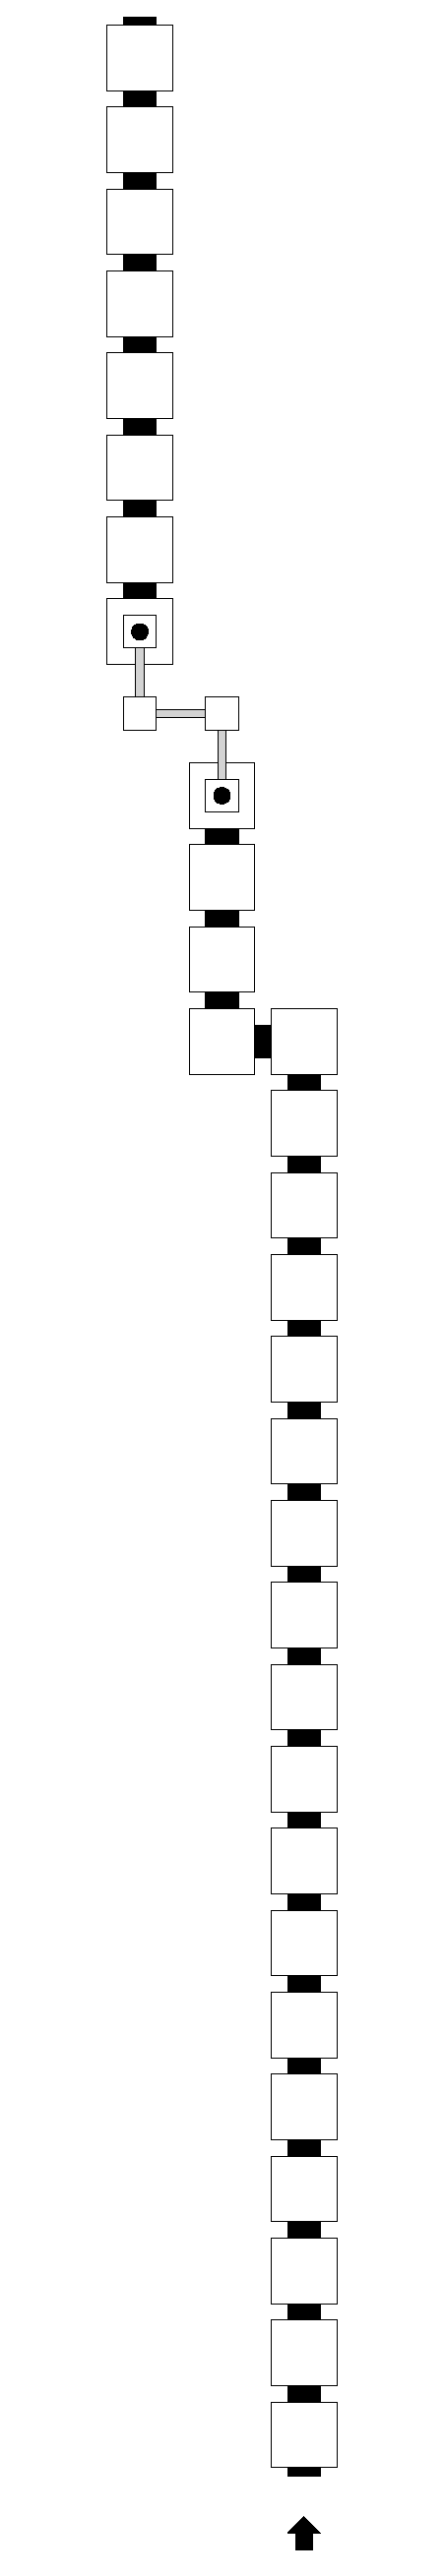
\includegraphics[width=0.45in]{warping_pre_warp_general}}}%
        ~
        \subcaptionbox{
            Digit 1 - general\\overview.
            The black tiles in this figure correspond to the gadget shown in subfigure~\subref{fig:pre_warp_general}.
            \label{fig:pre_warp_1_op_overview}
        }{\makebox[0.24\textwidth][c]{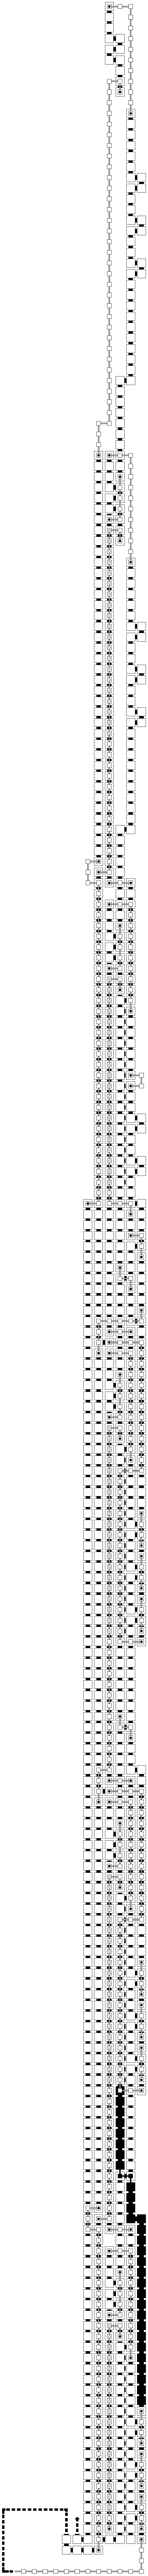
\includegraphics[width=0.45in]{overviews/general/pre_warp_1_op}}}%
        ~
        \subcaptionbox{
            Digit 2 - general\\overview.
            The black tiles in this figure correspond to the gadget shown in subfigure~\subref{fig:pre_warp_general}.
            \label{fig:pre_warp_2_op_overview}
        }{\makebox[0.24\textwidth][c]{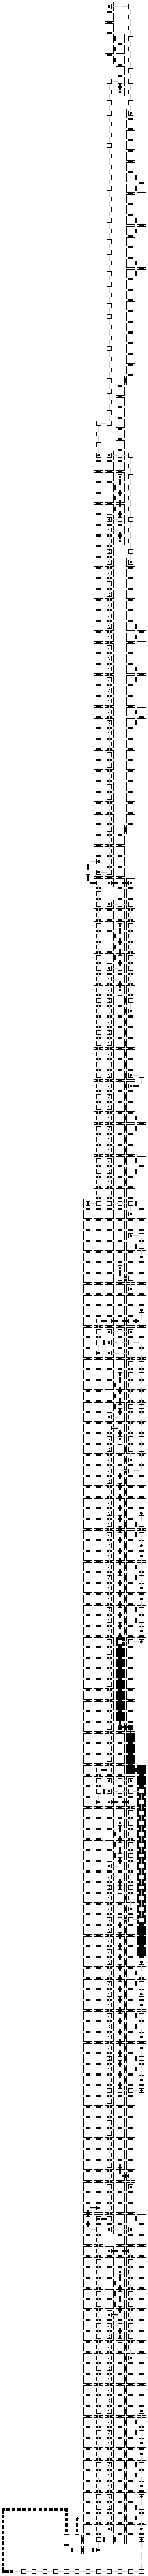
\includegraphics[width=0.45in]{overviews/general/pre_warp_2_op}}}%
        ~
        \subcaptionbox{
            Digit 3 - general\\overview.
            The black tiles in this figure correspond to the gadget shown in subfigure~\subref{fig:pre_warp_general}.
            \label{fig:pre_warp_3_op_overview}
        }{\makebox[0.24\textwidth][c]{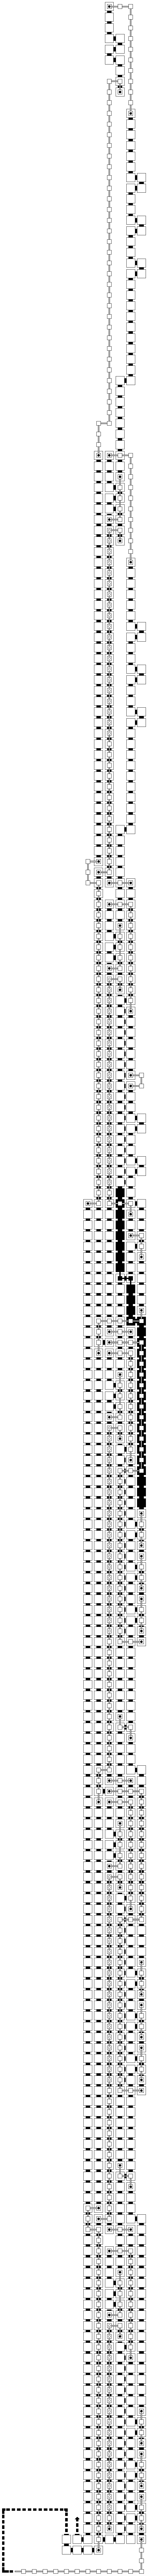
\includegraphics[width=0.45in]{overviews/general/pre_warp_3_op}}}%
        ~
    \end{figure}
    \begin{figure}[H]\ContinuedFloat
        \centering
        \subcaptionbox{
            Digit 1 - case 1.
            \label{fig:pre_warp_1_op_msr_msd}
        }{\makebox[0.24\textwidth][c]{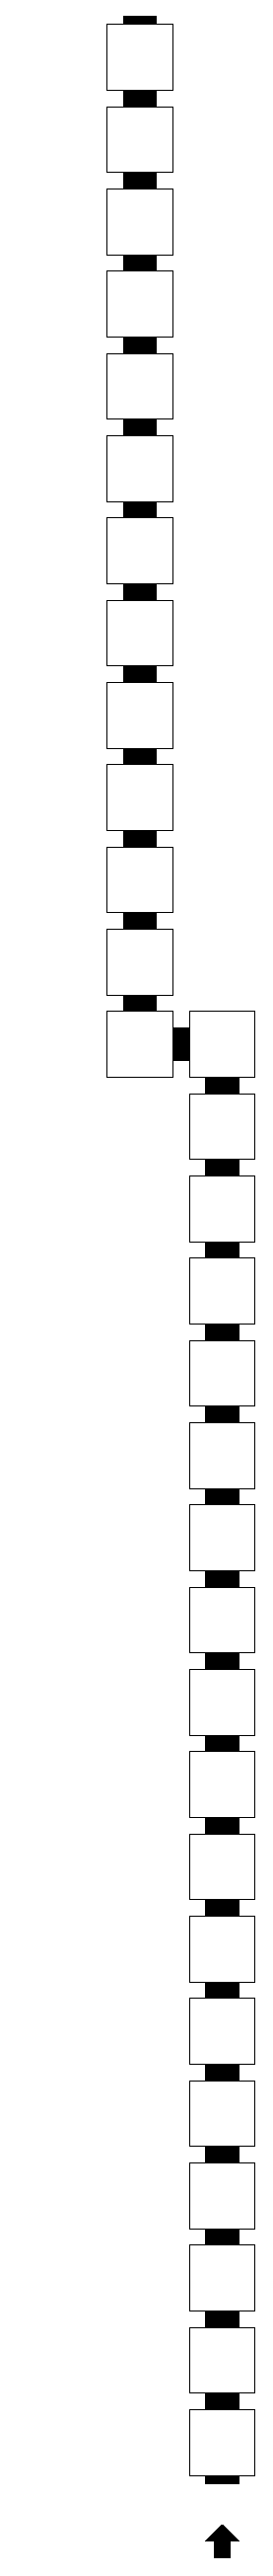
\includegraphics[width=0.45in]{warping_pre_warp_case1_digit1_msr}}}%
        ~
        \subcaptionbox{
            Digit 1 - case 1 overview.
            The black tiles in this figure correspond to the gadget shown in subfigure~\subref{fig:pre_warp_1_op_msr_msd}.
            \label{fig:pre_warp_1_op_msr_msd_overview}
        }{\makebox[0.24\textwidth][c]{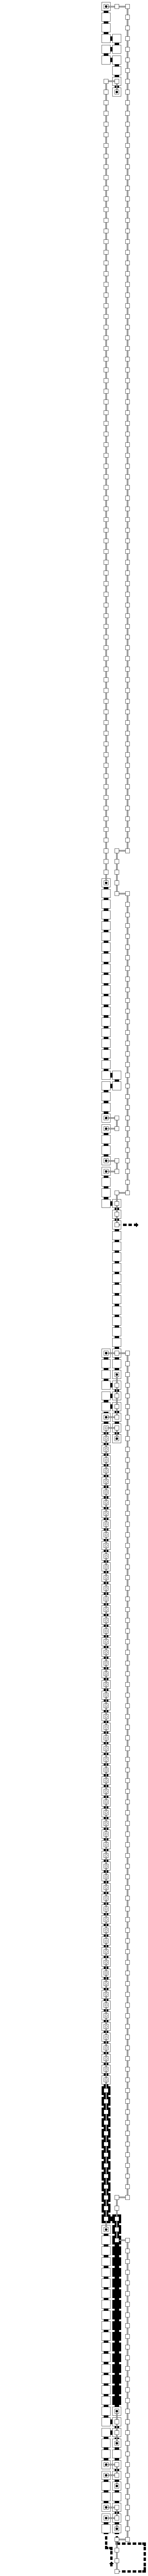
\includegraphics[width=0.45in]{overviews/case1/pre_warp_1_op_msr_msd}}}%
        ~
        \subcaptionbox{
            Digit 1 - case 2.
            \label{fig:pre_warp_1_op_msr}
        }{\makebox[0.24\textwidth][c]{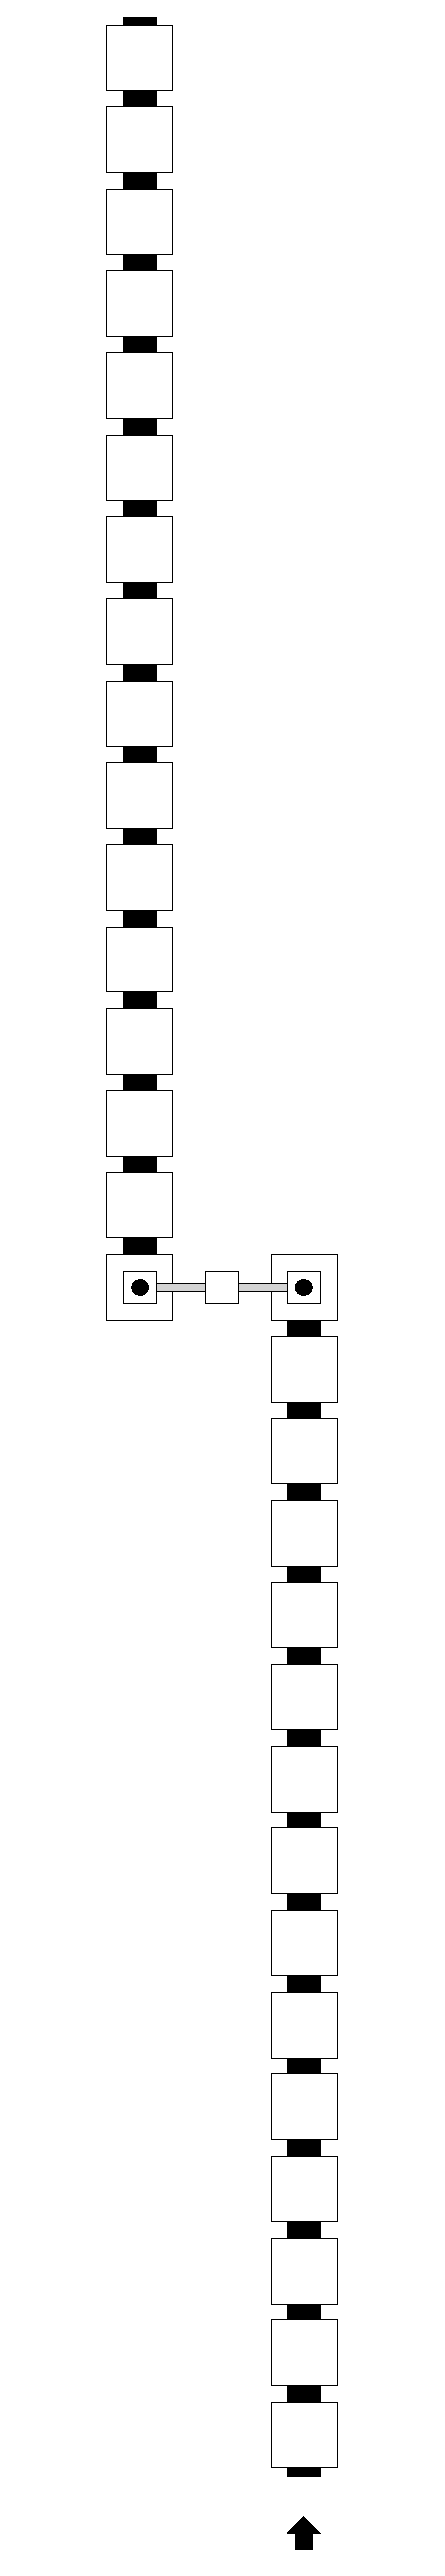
\includegraphics[width=0.45in]{warping_pre_warp_case2_digit1_msr}}}%
        ~
        \subcaptionbox{
            Digit 1 - case 2 overview.
            The black tiles in this figure correspond to the gadget shown in subfigure~\subref{fig:pre_warp_1_op_msr}.
            \label{fig:pre_warp_1_op_msr_overview}
        }{\makebox[0.24\textwidth][c]{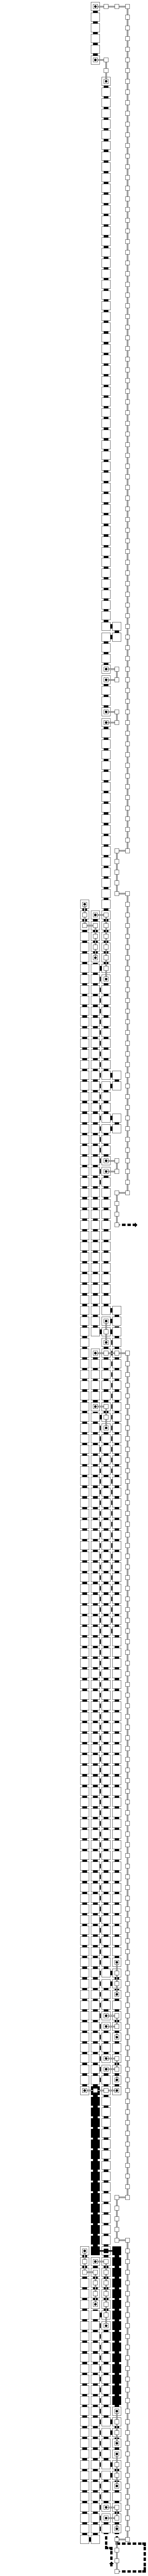
\includegraphics[width=0.45in]{overviews/case2/pre_warp_1_op_msr}}}%
        ~
    \end{figure}

    \begin{figure}[H]\ContinuedFloat
        \centering
        \subcaptionbox{
            Digit 2 - case 2.
            \label{fig:pre_warp_2_op_msr_msd}
        }{\makebox[0.24\textwidth][c]{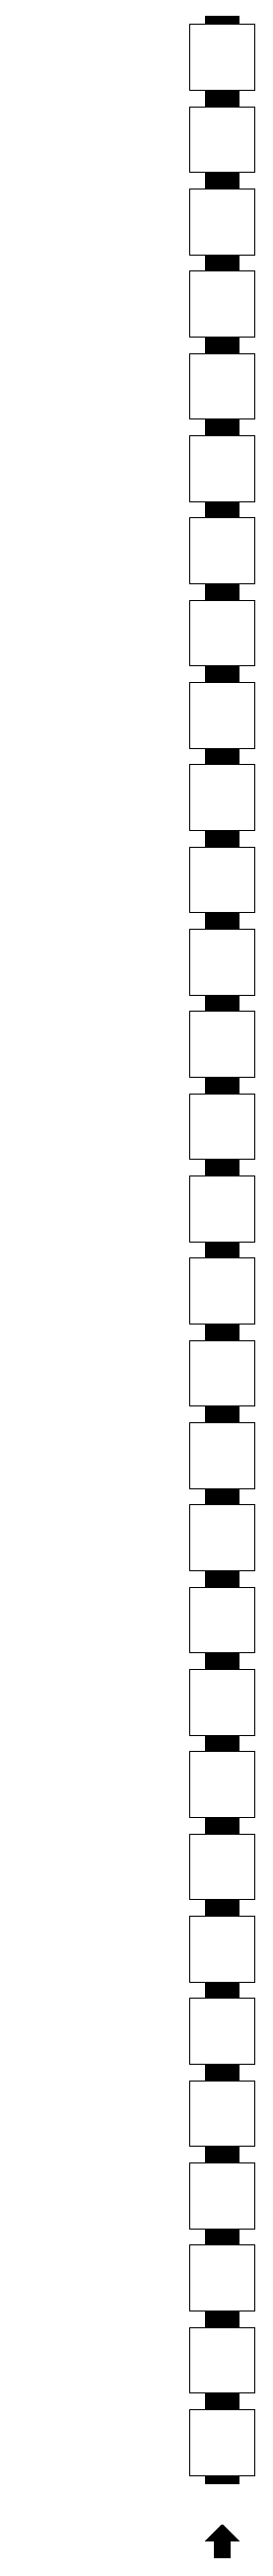
\includegraphics[width=0.45in]{warping_pre_warp_case2_digit2_msr}}}%
        ~
        \subcaptionbox{
            Digit 2 - case 2 overview.
            The black tiles in this figure correspond to the gadget shown in subfigure~\subref{fig:pre_warp_2_op_msr_msd}.
            \label{fig:pre_warp_2_op_msr_msd_overview}
        }{\makebox[0.24\textwidth][c]{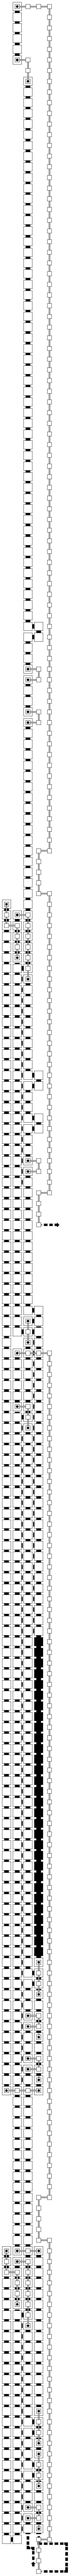
\includegraphics[width=0.45in]{overviews/case2/pre_warp_2_op_msr_msd}}}%
        ~
        \caption{\label{fig:pre_warp_gadgets} The {\prewarp} gadgets. }
    \end{figure}


    \item {\firstwarp}: The idea of the {\firstwarp} gadget is to transport the information read\\
        by the {\cread} gadgets, usually across a distance  $O(\log m)$. We do this using a single tile that
        assembles an infinite line in the north direction, and has one unique glue either in the
        east direction or west direction. This unique glue will at some point later in the assembly, that is
        determined by earlier parts of the assembly, no longer be blocked. When this occurs, it can
        finally attach to the {\warpbridge} gadget (except in a few special cases). This process signifies the ``waking up'' of the
        {\firstwarp} gadgets. When this gadget wakes up, it must also be blocked in the north direction, which
        prevents a truly infinite line from assembling. The geometry required for this process is guarenteed
        to be in place by earlier-assembled {\dtop} gadgets.

        For each $u \in \{0, 1\}^l$, and each $\inc \in \{ {\tt increment, copy } \}$:
        \begin{itemize}

            \item For each $i = 1,2,3$: create
            $\begin{aligned}[t]
                \firstwarp(& \left\langle {\tt FirstWarp},  i, u, \inc \right\rangle,\\  % South
                           & \left\langle {\tt FirstWarp},  i, u, \inc \right\rangle,\\  % North
                           & \left\langle {\tt WarpBridge}, i, u, \inc \right\rangle \;) % East
            \end{aligned}$\\ from the single tile gadget, shown in Figure~\ref{fig:first_warp_1_op_overview}
                             if $i = 1$ or Figure~\ref{fig:first_warp_2_op_overview} if $i = 2$, otherwise from
                             Figure~\ref{fig:first_warp_3_op_overview} if $i = 3$.
            \vspace{.5cm}

            \item Create
            $\begin{aligned}[t]
                \firstwarp(& \left\langle {\tt FirstWarp}, 1, u, \inc, {\tt msr} \right\rangle, \\ % South
                           & \left\langle {\tt FirstWarp}, 1, u, \inc, {\tt msr} \right\rangle, \\ % North
                           & \left\langle {\tt PostWarp},  1, u, \inc, {\tt msr} \right\rangle \;) % East
            \end{aligned}$\\ from the single tile gadget shown in Figure~\ref{fig:first_warp_1_op_msr_overview}.
            \vspace{.5cm}

            \item Create
            $\begin{aligned}[t]
                \firstwarp(& \left\langle {\tt FirstWarp}, 1, u, \inc, {\tt msr}, {\tt msd} \right\rangle, \\ % South
                           & \left\langle {\tt FirstWarp}, 1, u, \inc, {\tt msr}, {\tt msd} \right\rangle, \\ % North
                           & \left\langle {\tt PostWarp},  1, u, \inc, {\tt msr}, {\tt msd} \right\rangle \;) % Up
            \end{aligned}$\\ from the single tile gadget shown in Figure~\ref{fig:first_warp_1_op_msr_msd_overview}.
            \vspace{.5cm}

            \item Create
            $\begin{aligned}[t]
                \firstwarp(& \left\langle {\tt FirstWarp},  2, u, \inc, {\tt msr}, {\tt msd} \right\rangle, \\ % South
                           & \left\langle {\tt FirstWarp},  2, u, \inc, {\tt msr}, {\tt msd} \right\rangle, \\ % North
                           & \left\langle {\tt WarpBridge}, 2, u, \inc, {\tt msr}, {\tt msd} \right\rangle \;) % West
            \end{aligned}$\\ from the single tile gadget shown in Figure~\ref{fig:first_warp_2_op_msr_msd_overview}.
            \vspace{.5cm}

            \item Create
            $\begin{aligned}[t]
                \firstwarp(& \left\langle {\tt FirstWarp},  3, u, \inc, {\tt msr}, {\tt msd} \right\rangle,\\  % South
                           & \left\langle {\tt FirstWarp},  3, u, \inc, {\tt msr}, {\tt msd} \right\rangle,\\  % North
                           & \left\langle {\tt WarpBridge}, 3, u, \inc, {\tt msr}, {\tt msd} \right\rangle \;) % East
            \end{aligned}$\\ from the single tile gadget shown in Figure~\ref{fig:first_warp_3_op_msr_msd_overview}.
            \vspace{.5cm}

        \end{itemize}
        \vspace{.5cm}

    \begin{figure}[H]
        \centering
        \subcaptionbox{
            Digit 1 - general\\ overview.
            \label{fig:first_warp_1_op_overview}
        }{\makebox[0.24\textwidth][c]{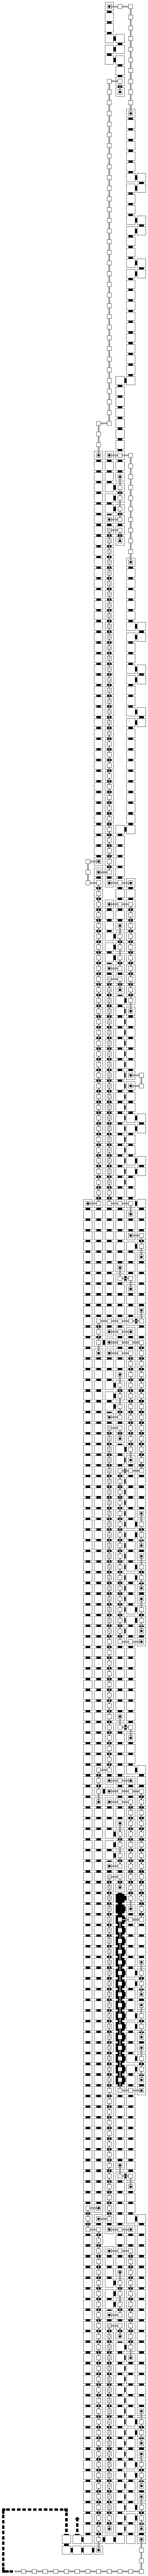
\includegraphics[width=0.45in]{overviews/general/first_warp_1_op}}}%
        ~
        \subcaptionbox{
            Digit 2 - general\\ overview.
            \label{fig:first_warp_2_op_overview}
        }{\makebox[0.24\textwidth][c]{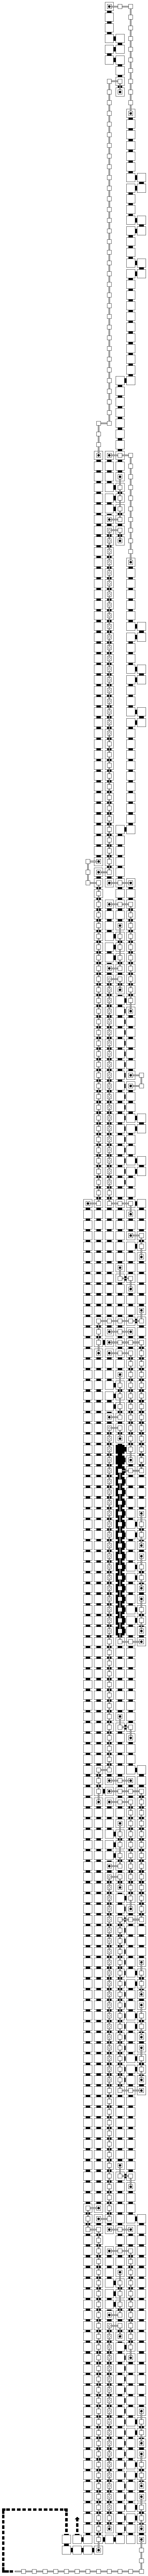
\includegraphics[width=0.45in]{overviews/general/first_warp_2_op}}}%
        ~
        \subcaptionbox{
            Digit 3 - general\\ overview.
            \label{fig:first_warp_3_op_overview}
        }{\makebox[0.24\textwidth][c]{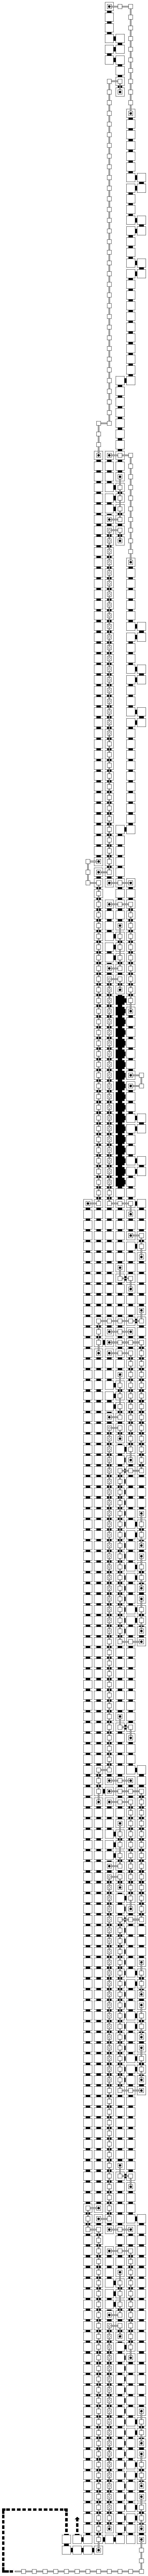
\includegraphics[width=0.45in]{overviews/general/first_warp_3_op}}}%
        ~
        \subcaptionbox{
            Digit 3 - general (seed) overview.
            \label{fig:first_warp_3_seed_op_overview}
        }{\makebox[0.24\textwidth][c]{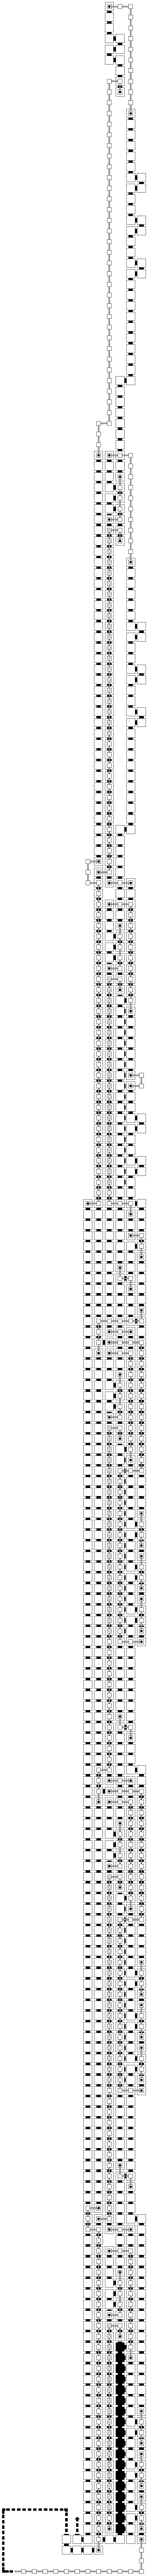
\includegraphics[width=0.45in]{overviews/general/first_warp_3_seed_op}}}%
        ~
    \end{figure}

    \begin{figure}[H]\ContinuedFloat
        \centering
        \subcaptionbox{
            Digit 1 - case 1 overview.
            \label{fig:first_warp_1_op_msr_msd_overview}
        }{\makebox[0.24\textwidth][c]{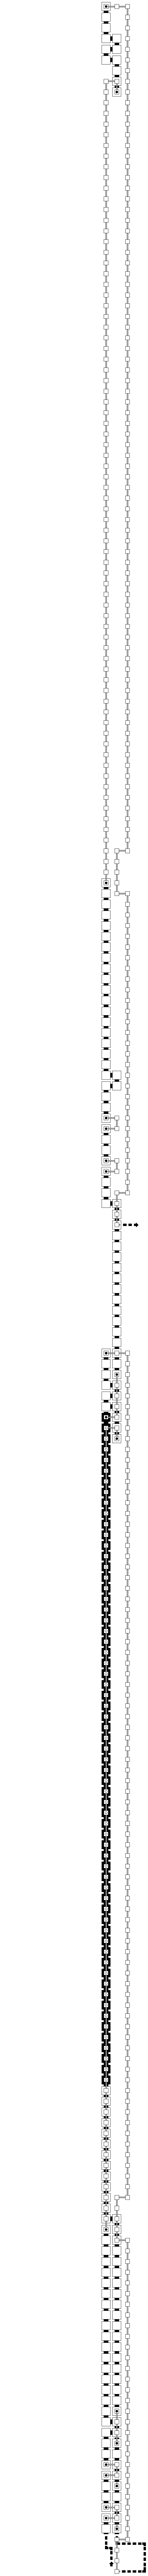
\includegraphics[width=0.45in]{overviews/case1/first_warp_1_op_msr_msd}}}%
        ~
        \subcaptionbox{
            Digit 1 - case 2 overview.
            \label{fig:first_warp_1_op_msr_overview}
        }{\makebox[0.24\textwidth][c]{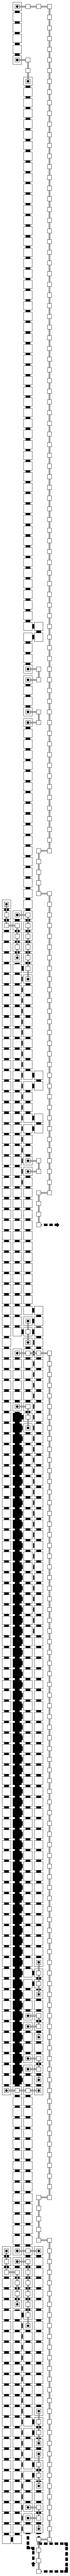
\includegraphics[width=0.45in]{overviews/case2/first_warp_1_op_msr}}}%
        ~
        \subcaptionbox{
            Digit 2 - case 2 overview.
            \label{fig:first_warp_2_op_msr_msd_overview}
        }{\makebox[0.24\textwidth][c]{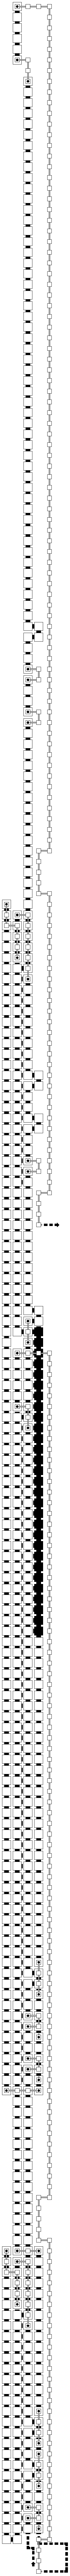
\includegraphics[width=0.45in]{overviews/case2/first_warp_2_op_msr_msd}}}%
        ~
        \subcaptionbox{
            Digit 3 - case 3 overview.
            \label{fig:first_warp_3_op_msr_msd_overview}
        }{\makebox[0.24\textwidth][c]{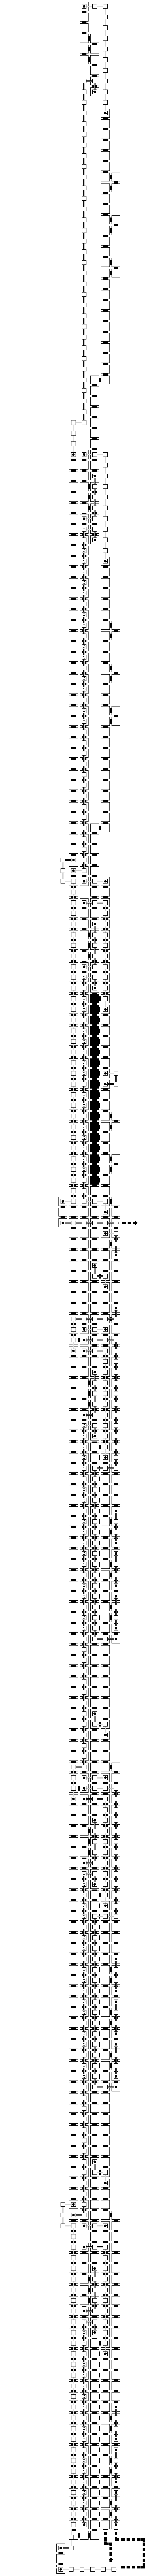
\includegraphics[width=0.45in]{overviews/case3/first_warp_3_op_msr_msd}}}%
        ~
        \caption{\label{fig:first_warp_gadgets_overviews} The {\firstwarp} gadget overviews.}
    \end{figure}


    \item {\warpbridge}: a {\warpbridge} gadget is a gadget which assembles when the {\firstwarp} gadget makes it
         to its final destination. The goal of the {\warpbridge} is to assemble a path from the end of the {\firstwarp}
         gadgets to the start of the {\secondwarp} gadgets. For digit 1 in cases 1 and 2, the {\warpbridge} is omitted
         from the {\warpunit}.

    For each $u \in \{0, 1\}^l$, and each $\inc \in \{ {\tt increment, copy } \}$:
    \begin{itemize}

        \item For each $i = 1,2,3$: create
        $\begin{aligned}[t]
            \warpbridge(& \left\langle {\tt WarpBridge}, i, u, \inc \right\rangle,
                          \left\langle {\tt SecondWarp}, i, u, \inc \right\rangle \;)
        \end{aligned}$ \\ from the general gadget in Figure~\ref{fig:warp_bridge_general}.
        \vspace{.5cm}

        \item Create
        $\begin{aligned}[t]
            \warpbridge(& \left\langle {\tt WarpBridge}, 2, u, \inc, {\tt msr}, {\tt msd} \right\rangle,
                          \left\langle {\tt SecondWarp}, 2, u, \inc, {\tt msr}, {\tt msd} \right\rangle \;)
        \end{aligned}$ \\ from the general gadget in Figure~\ref{fig:warp_bridge_2_op_msr_msd}.
        \vspace{.5cm}

        \item Create
        $\begin{aligned}[t]
            \warpbridge(& \left\langle {\tt WarpBridge}, 3, u, \inc, {\tt msr}, {\tt msd} \right\rangle,
                          \left\langle {\tt SecondWarp}, 3, u, \inc, {\tt msr}, {\tt msd} \right\rangle \;)
        \end{aligned}$ \\ from the general gadget in Figure~\ref{fig:warp_bridge_general}.
        \vspace{.5cm}
    \end{itemize}


    \begin{figure}[H]
        \centering
        \subcaptionbox{
            Digits 1, 2, \& 3 general.
            \label{fig:warp_bridge_general}
        }{\makebox[0.24\textwidth][c]{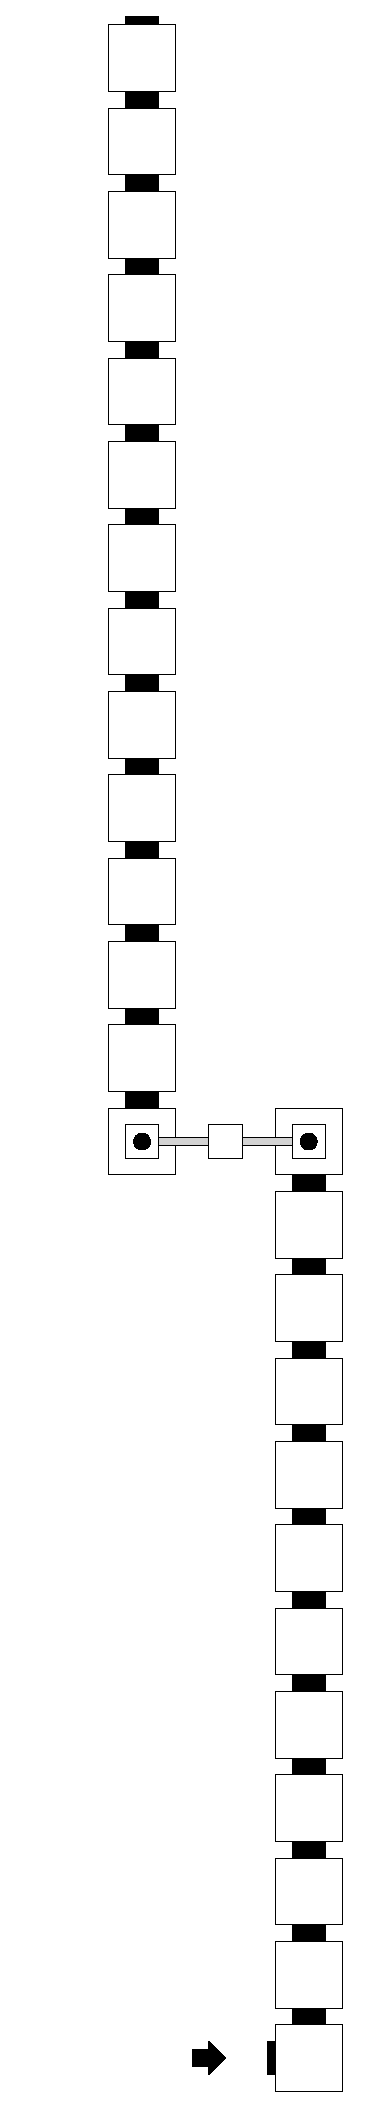
\includegraphics[width=0.45in]{warping_warp_bridge_general}}}%
        ~
        \subcaptionbox{
            Digit 1 - general\\ overview.
            The black tiles in this figure correspond to the gadget shown in subfigure~\subref{fig:warp_bridge_general}.
            \label{fig:warp_bridge_1_op_overview}
        }{\makebox[0.24\textwidth][c]{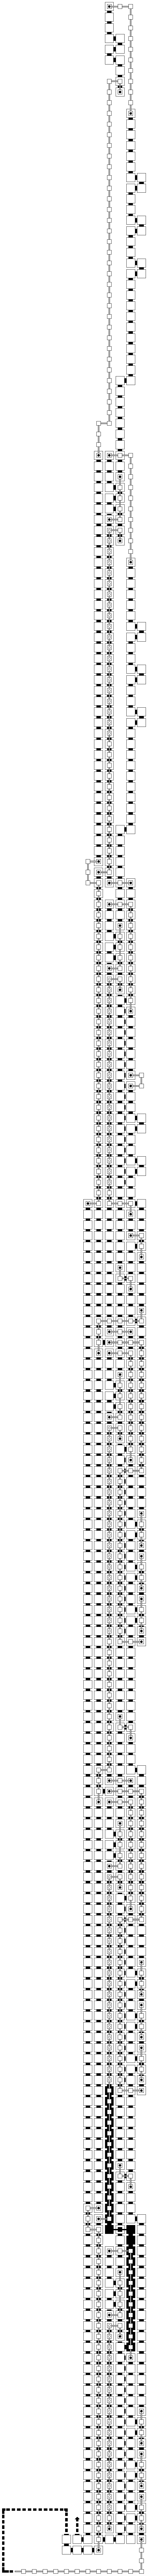
\includegraphics[width=0.45in]{overviews/general/warp_bridge_1_op}}}%
        ~
        \subcaptionbox{
            Digit 2 - general\\ overview.
            The black tiles in this figure correspond to the gadget shown in subfigure~\subref{fig:warp_bridge_general}.
            \label{fig:warp_bridge_2_op_overview}
        }{\makebox[0.24\textwidth][c]{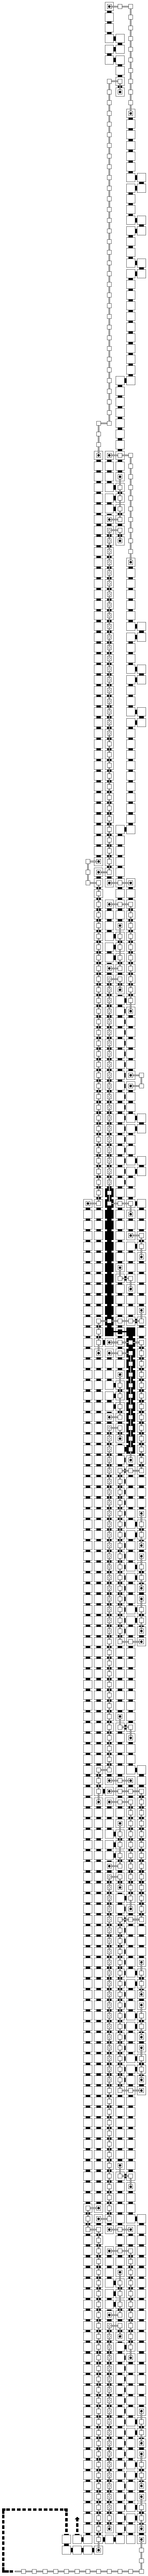
\includegraphics[width=0.45in]{overviews/general/warp_bridge_2_op}}}%
        ~
        \subcaptionbox{
            Digit 2 - general (seed) overview.
            The black tiles in this figure correspond to the gadget shown in subfigure~\subref{fig:warp_bridge_general}.
            \label{fig:warp_bridge_2_seed_op_overview}
        }{\makebox[0.24\textwidth][c]{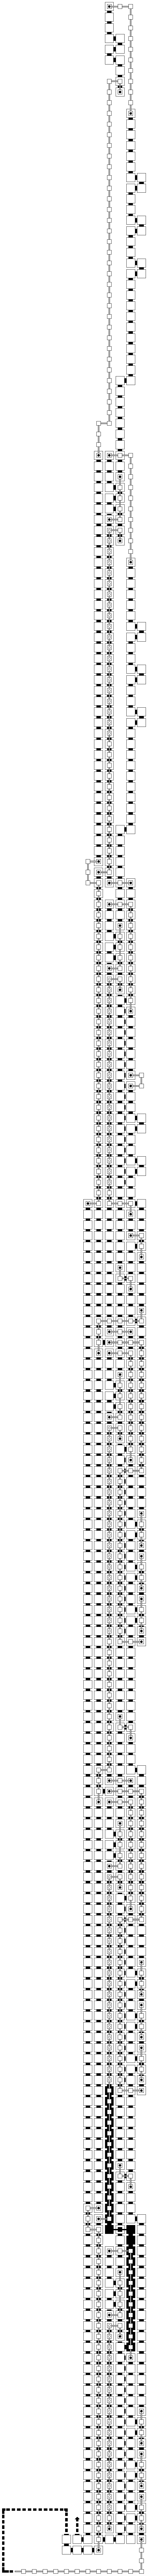
\includegraphics[width=0.45in]{overviews/general/warp_bridge_2_seed_op}}}%
        ~
    \end{figure}
    \begin{figure}[H]\ContinuedFloat
        \centering
        \subcaptionbox{
            Digit 3 - general\\ overview.
            The black tiles in this figure correspond to the gadget shown in subfigure~\subref{fig:warp_bridge_general}.
            \label{fig:warp_bridge_3_op_overview}
        }{\makebox[0.24\textwidth][c]{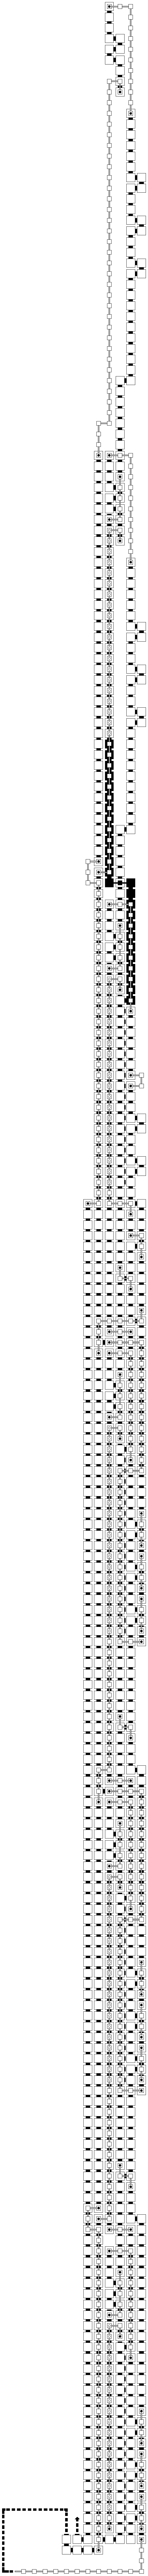
\includegraphics[width=0.45in]{overviews/general/warp_bridge_3_op}}}%
        ~
        \subcaptionbox{
            Digit 3 - general (seed) overview.
            The black tiles in this figure correspond to the gadget shown in subfigure~\subref{fig:warp_bridge_general}.
            \label{fig:warp_bridge_3_seed_op_overview}
        }{\makebox[0.24\textwidth][c]{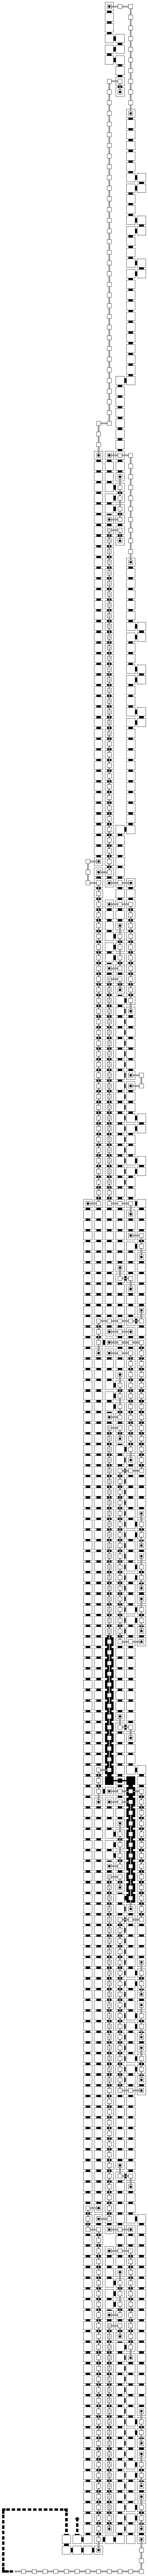
\includegraphics[width=0.45in]{overviews/general/warp_bridge_3_seed_op}}}%
        ~
        \subcaptionbox{
            Digit 2 - case 2.
            \label{fig:warp_bridge_2_op_msr_msd}
        }{\makebox[0.24\textwidth][c]{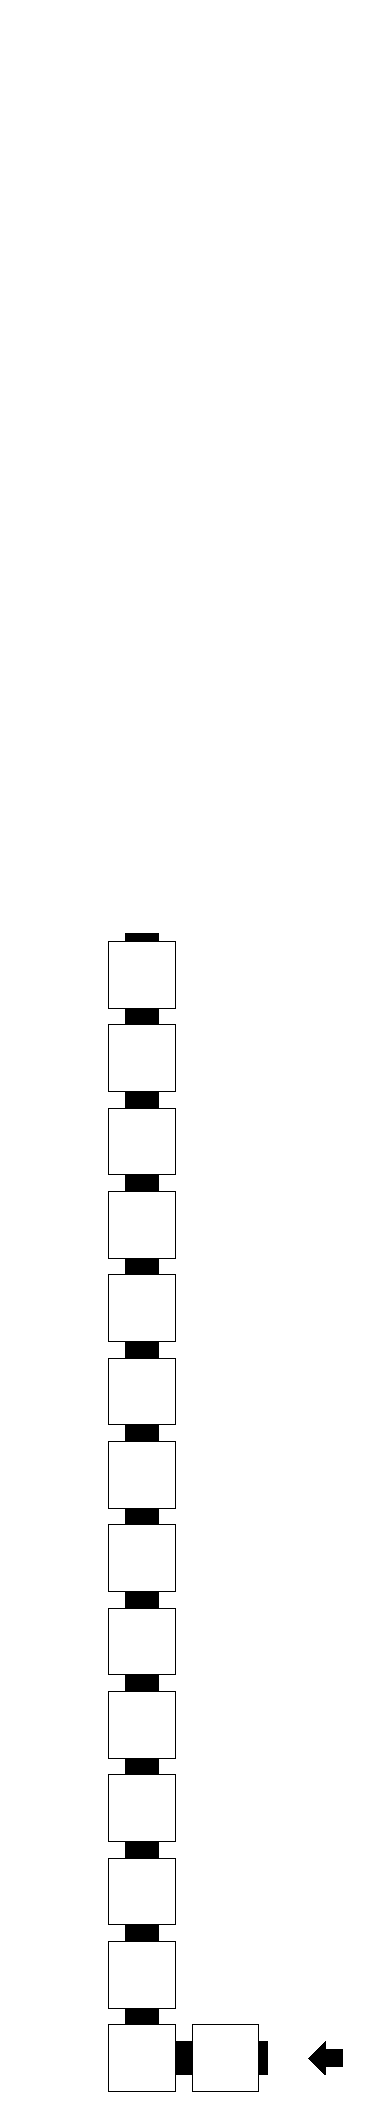
\includegraphics[width=0.45in]{warping_warp_bridge_case2_digit2_msr}}}%
        ~
        \subcaptionbox{
            Digit 2 - case 2 overview.
            The black tiles in this figure correspond to the gadget shown in subfigure~\subref{fig:warp_bridge_2_op_msr_msd}.
            \label{fig:warp_bridge_2_op_msr_msd_overview}
        }{\makebox[0.24\textwidth][c]{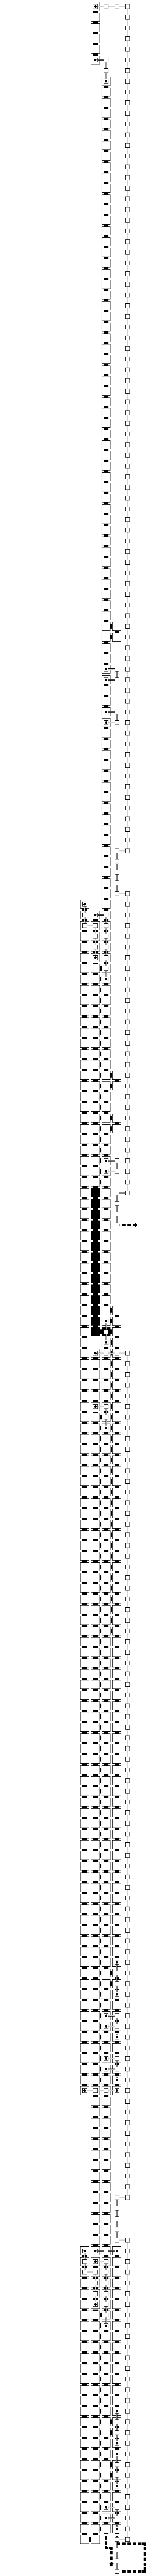
\includegraphics[width=0.45in]{overviews/case2/warp_bridge_2_op_msr_msd}}}%
        ~
        \caption{\label{fig:warp_bridge_gadgets_overviews} The {\warpbridge} gadgets.}
    \end{figure}

    \item {\secondwarp}:
    Similar to the {\firstwarp} gadgets, the idea of the {\secondwarp} gadget is to
    also to transport the information read by the {\cread} gadgets. We do this using a single tile that
    assembles an infinite line in the north direction, and has one unique glue either in the
    east direction or up direction. This unique glue will at some point later in the assembly, that is
    determined by earlier parts of the assembly, no longer be blocked. When this occurs, it can
    finally attach to the {\postwarp} gadget. This process signifies the ``waking up'' of the
    {\secondwarp} gadgets. When this gadget wakes up, it must also be blocked in the north direction, which
    prevent a truly infinite line from assembling. The geometry required for this process is guarenteed
    to be in place by earlier-assembled {\dtop} gadgets.


    For each $u \in \{0, 1\}^l$, and each $\inc \in \{ {\tt increment, copy } \}$:
    \begin{itemize}
        \item For each $i = 1, 2, 3$: \\
        Create
        $\begin{aligned}[t]
            \secondwarp(& \left\langle {\tt SecondWarp}, i, u, \inc \right\rangle,     % South
                          \left\langle {\tt SecondWarp}, i, u, \inc \right\rangle,     % North
                          \left\langle {\tt PostWarp},   i, u, \inc \right\rangle \;)  % Up
        \end{aligned}$\\ from the single tile gadget, shown in Figure~\ref{fig:second_warp_1_op_overview}
                         if $i = 1$ or Figure~\ref{fig:second_warp_2_op_overview} if $i = 2$, otherwise from
                         Figure~\ref{fig:second_warp_3_op_overview} if $i = 3$.
        \vspace{0.5cm}

        \item Create
        $\begin{aligned}[t]
            \secondwarp(& \left\langle {\tt SecondWarp}, 2, u, \inc, {\tt msr}, {\tt msd} \right\rangle, \\ % South
                        & \left\langle {\tt SecondWarp}, 2, u, \inc, {\tt msr}, {\tt msd} \right\rangle, \\ % North
                        & \left\langle {\tt PostWarp},   2, u, \inc, {\tt msr}, {\tt msd} \right\rangle \;) % East
        \end{aligned}$\\ from the single tile gadget shown in Figure~\ref{fig:second_warp_2_op_msr_msd_overview}.
        \vspace{0.5cm}

        \item Create
        $\begin{aligned}[t]
            \secondwarp(& \left\langle {\tt SecondWarp}, 3, u, \inc, {\tt msr}, {\tt msd} \right\rangle, \\ % South
                        & \left\langle {\tt SecondWarp}, 3, u, \inc, {\tt msr}, {\tt msd} \right\rangle, \\ % North
                        & \left\langle {\tt PostWarp},   3, u, \inc, {\tt msr}, {\tt msd} \right\rangle \;) % Up
        \end{aligned}$\\ from the single tile gadget shown in Figure~\ref{fig:second_warp_3_op_msr_msd_overview}.
    \end{itemize}

    \begin{figure}[H]
        \centering
        \subcaptionbox{
            Digit 1 - general\\ overview.
            \label{fig:second_warp_1_op_overview}
        }{\makebox[0.24\textwidth][c]{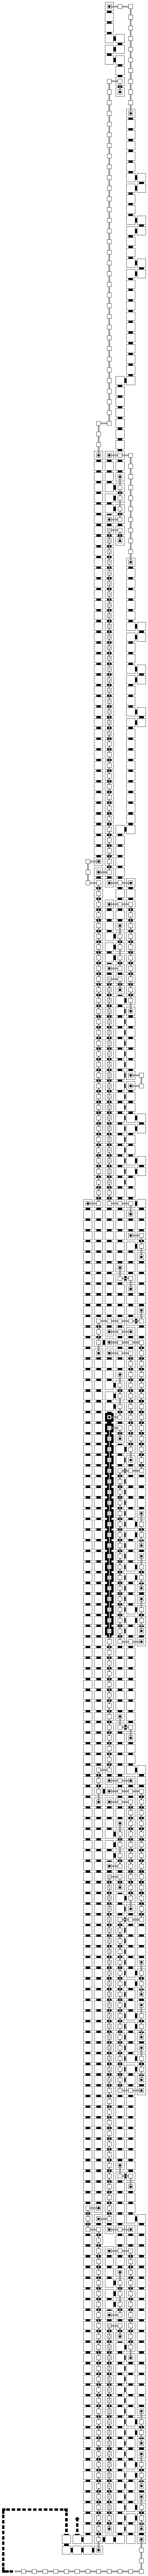
\includegraphics[width=0.45in]{overviews/general/second_warp_1_op}}}%
        ~
        \subcaptionbox{
            Digit 2 - general\\ overview.
            \label{fig:second_warp_2_op_overview}
        }{\makebox[0.24\textwidth][c]{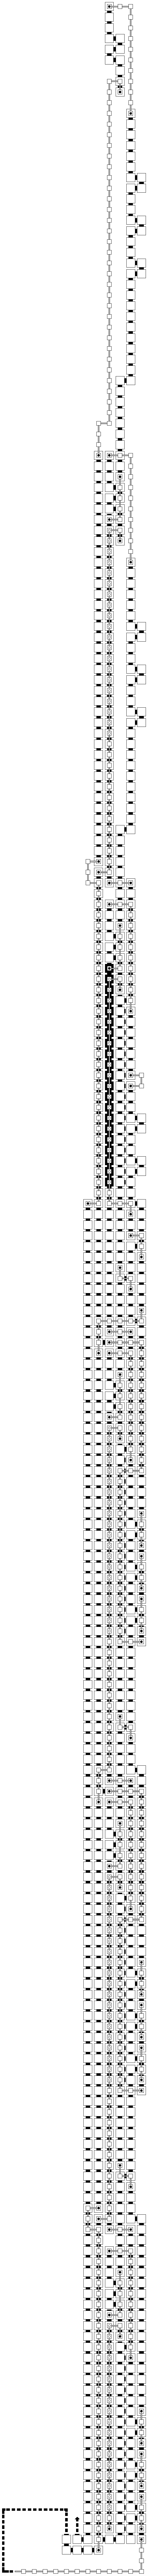
\includegraphics[width=0.45in]{overviews/general/second_warp_2_op}}}%
        ~
        \subcaptionbox{
            Digit 3 - general\\ overview.
            \label{fig:second_warp_3_op_overview}
        }{\makebox[0.24\textwidth][c]{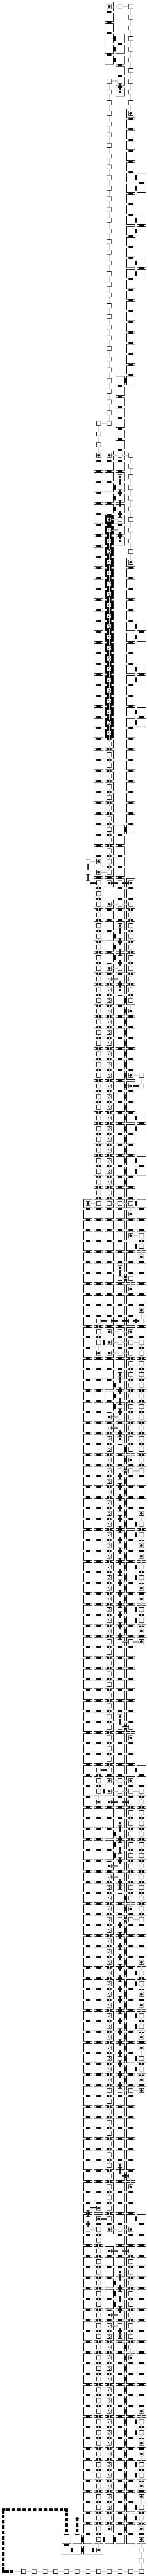
\includegraphics[width=0.45in]{overviews/general/second_warp_3_op}}}%
        ~
        \subcaptionbox{
            Digit 2 - general (seed) overview.
            \label{fig:second_warp_2_seed_op_overview}
        }{\makebox[0.24\textwidth][c]{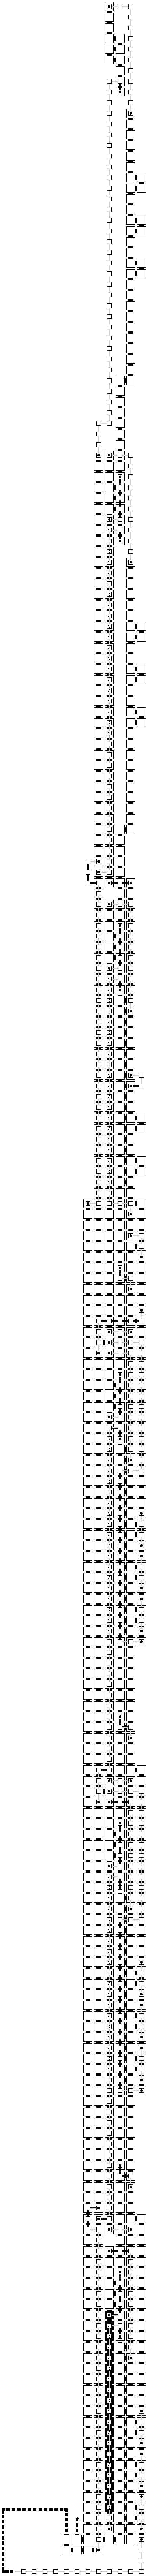
\includegraphics[width=0.45in]{overviews/general/second_warp_2_seed_op}}}%
        ~
    \end{figure}
    \begin{figure}[H]\ContinuedFloat
        \centering
        \subcaptionbox{
            Digit 3 - general (seed) overview.
            \label{fig:second_warp_3_seed_op_overview}
        }{\makebox[0.24\textwidth][c]{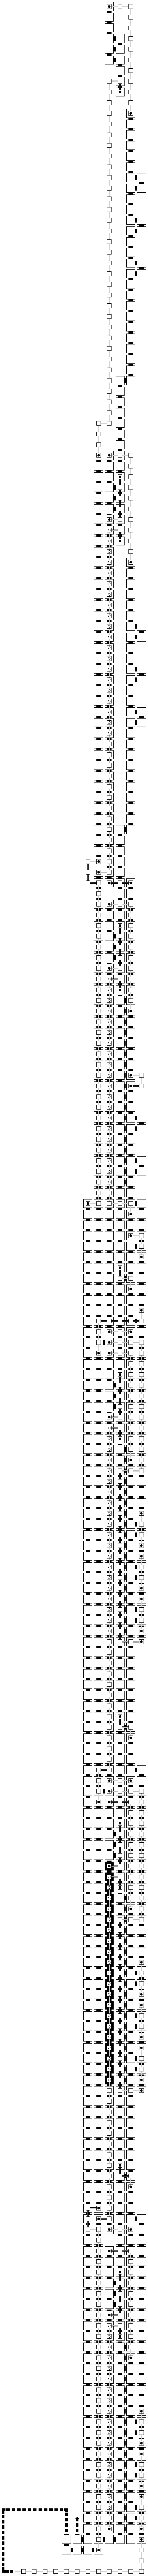
\includegraphics[width=0.45in]{overviews/general/second_warp_3_seed_op}}}%
        ~
        \subcaptionbox{
            Digit 2 - case 2 overview.
            \label{fig:second_warp_2_op_msr_msd_overview}
        }{\makebox[0.24\textwidth][c]{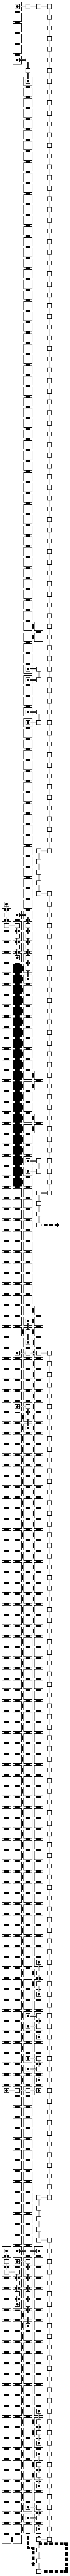
\includegraphics[width=0.45in]{overviews/case2/second_warp_2_op_msr_msd}}}%
        ~
        \subcaptionbox{
            Digit 2 - case 2 (seed) overview.
            \label{fig:second_warp_2_seed_op_msr_msd_overview}
        }{\makebox[0.24\textwidth][c]{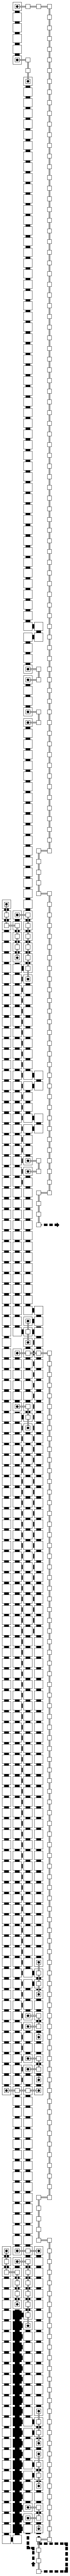
\includegraphics[width=0.45in]{overviews/case2/second_warp_2_seed_op_msr_msd}}}%
        ~
        \subcaptionbox{
            Digit 3 - case 3 overview.
            \label{fig:second_warp_3_op_msr_msd_overview}
        }{\makebox[0.24\textwidth][c]{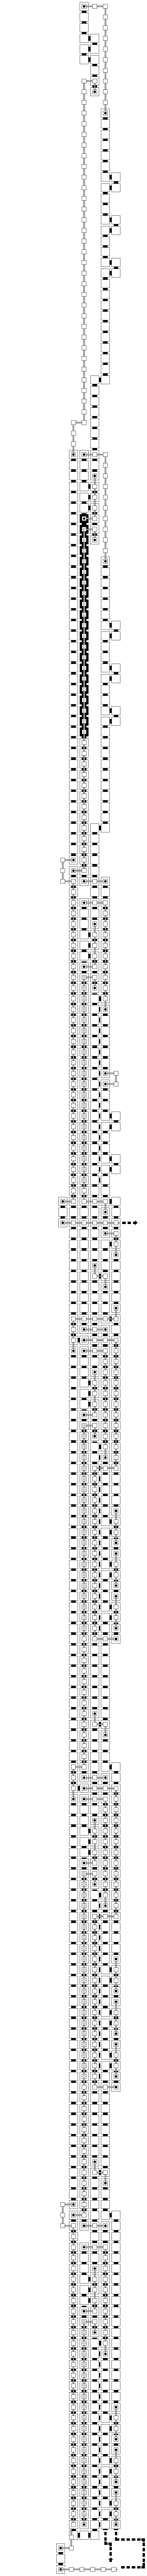
\includegraphics[width=0.45in]{overviews/case3/second_warp_3_op_msr_msd}}}%
        ~
        \caption{\label{fig:second_warp_gadgets_overviews} The {\secondwarp} gadget overviews.}
    \end{figure}


    \item {\postwarp}: The {\postwarp} gadget is final gadget to assemble in the {\warpunit}. The idea of this
    gadget is to assemble from wherever the last warping tiles ``wake up'', forming a path that ends where the
    next digit needs to start being written.

    \begin{itemize}
       \item For each $i = 1,2,3$: create\\
        $\begin{aligned}[t]
            \postwarp(& \left \langle {\tt PostWarp},     i, u, \inc \right\rangle,    % Down
                        \left \langle {\tt CounterWrite}, i, u, \inc \right\rangle \;) % North
        \end{aligned}$ \\
        from the general gadget shown in Figure~\ref{fig:post_warp_1_op} if $i = 1$,
        or Figure~\ref{fig:post_warp_2or3_op} if $ i = 2$ or $i = 3$.
        \vspace{.5cm}


        \item Create
        $\begin{aligned}[t]
            \postwarp(& \left \langle {\tt PostWarp},     1, u, \inc, {\tt msr} \right\rangle,    % West
                        \left \langle {\tt CounterWrite}, 1, u, \inc, {\tt msr} \right\rangle \;) % North
        \end{aligned}$ \\
        from the general gadget in Figure~\ref{fig:post_warp_1_op_msr}.
        \vspace{.5cm}

        \item For each $i=1,2,3$: create\\
        $\begin{aligned}[t]
            \postwarp(& \left \langle {\tt PostWarp},     i, u, \inc, {\tt msr}, {\tt msd} \right\rangle,    % Down if i=1 or i=3, West if i=2
                        \left \langle {\tt CounterWrite}, i, u, \inc, {\tt msr}, {\tt msd} \right\rangle \;) % North
        \end{aligned}$ \\
        from the general gadget shown in Figure~\ref{fig:post_warp_1_op_msr_msd} if $i = 1$, or
        Figure~\ref{fig:post_warp_2_op_msr_msd} if $i = 2$, or Figure~\ref{fig:post_warp_2or3_op} if $i = 3$.
        \vspace{.5cm}

    \end{itemize}

    \begin{figure}[H]
        \centering
        \subcaptionbox{
            Digit 1 - general.
            \label{fig:post_warp_1_op}
        }{\makebox[0.24\textwidth][c]{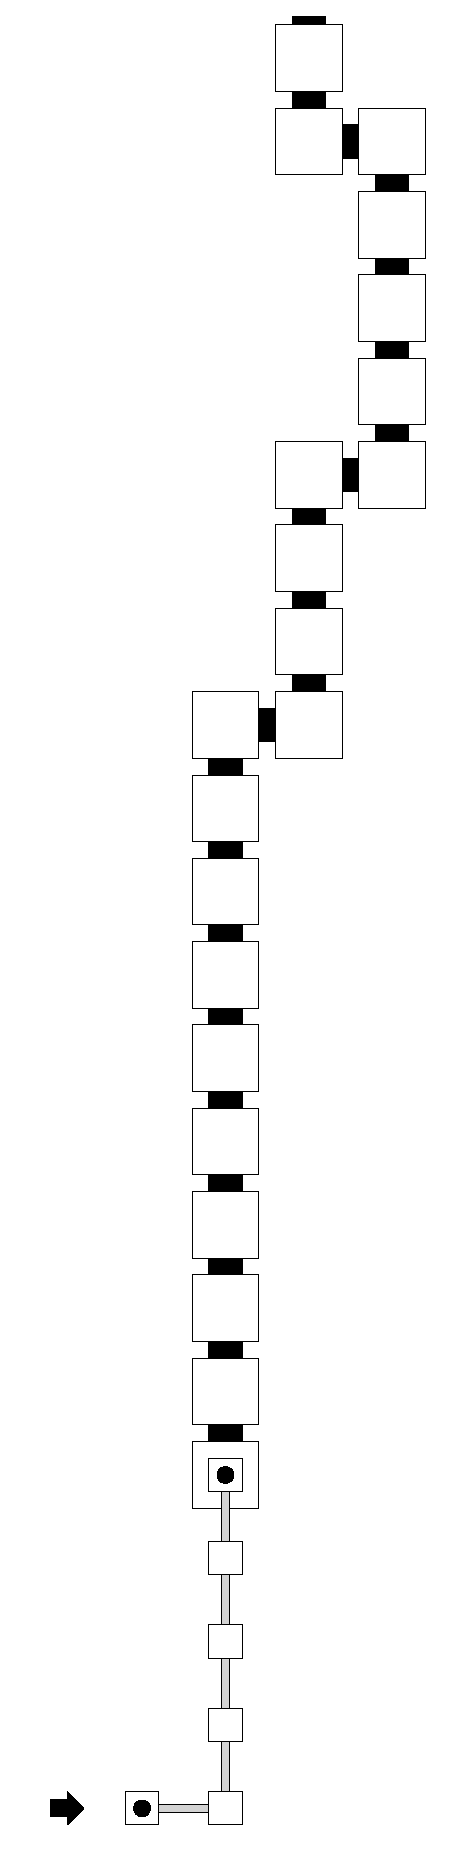
\includegraphics[width=0.45in]{warping_post_warp_general_digit1}}}%
        ~
        \subcaptionbox{
            Digit 1 - general\\overview.
            The black tiles in this figure correspond to the gadget shown in subfigure~\subref{fig:post_warp_1_op}.
            \label{fig:post_warp_1_op_overview}
        }{\makebox[0.24\textwidth][c]{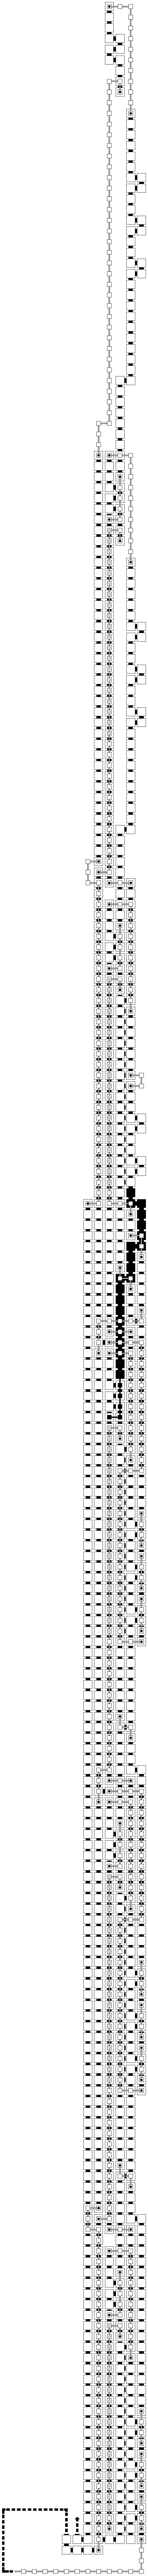
\includegraphics[width=0.45in]{overviews/general/post_warp_1_op}}}%
        ~
        \subcaptionbox{
            Digit 2 \& 3 - general.
            \label{fig:post_warp_2or3_op}
        }{\makebox[0.24\textwidth][c]{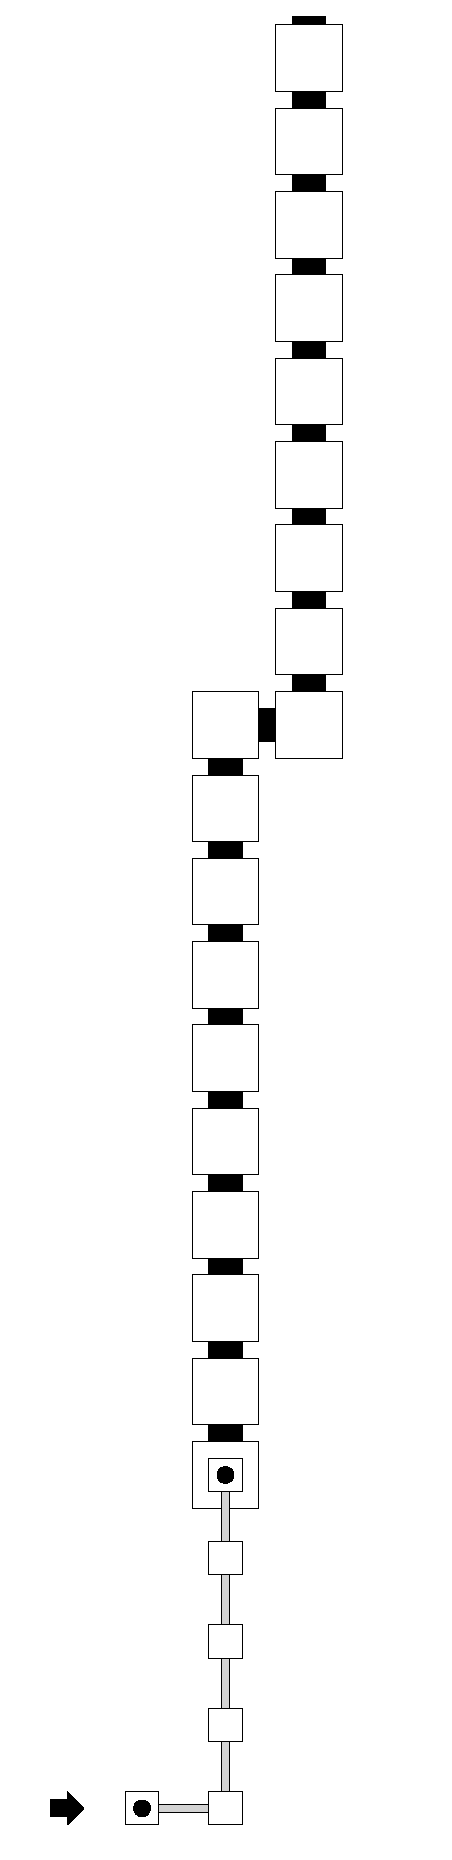
\includegraphics[width=0.45in]{warping_post_warp_general_digit2and3}}}%
        ~
        \subcaptionbox{
            Digit 2 - general\\overview.
            The black tiles in this figure correspond to the gadget shown in subfigure~\subref{fig:post_warp_2or3_op}.
            \label{fig:post_warp_2_op_overview}
        }{\makebox[0.24\textwidth][c]{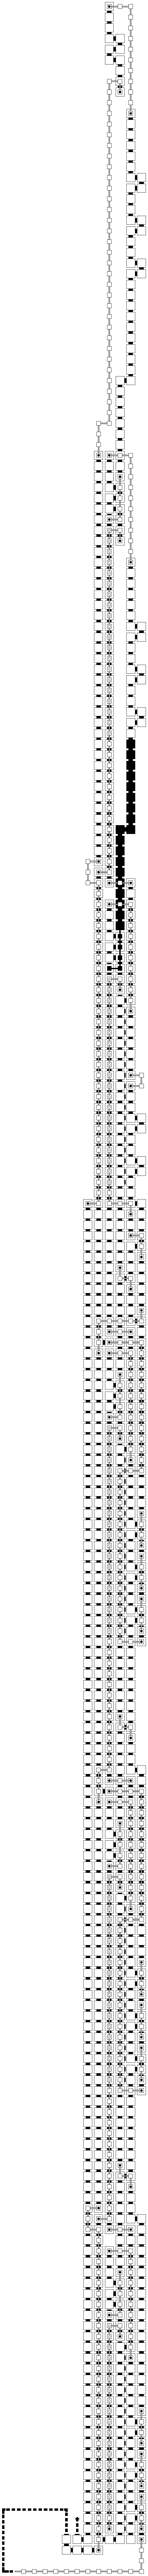
\includegraphics[width=0.45in]{overviews/general/post_warp_2_op}}}%
        ~
    \end{figure}
    \begin{figure}[H]\ContinuedFloat
        \centering
        \subcaptionbox{
            Digit 2 - general (seed) overview.
            The black tiles in this figure correspond to the gadget shown in subfigure~\subref{fig:post_warp_2or3_op}.
            \label{fig:post_warp_2_seed_op_overview}
        }{\makebox[0.24\textwidth][c]{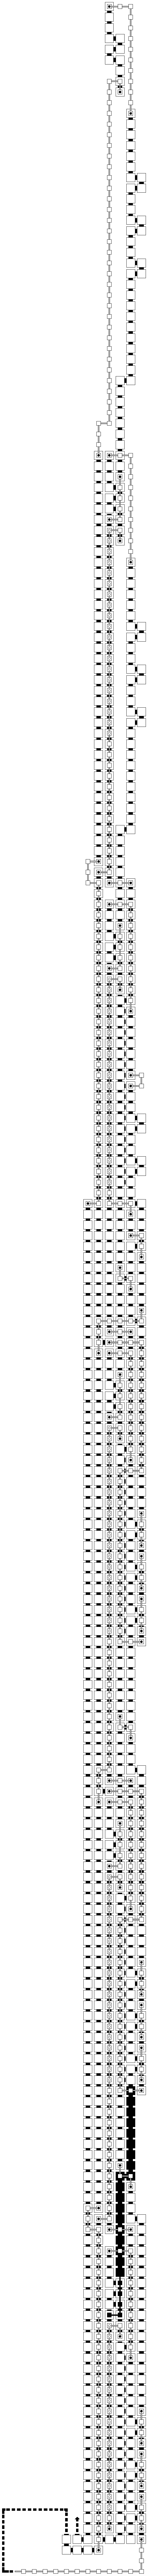
\includegraphics[width=0.45in]{overviews/general/post_warp_2_seed_op}}}%
        ~
        \subcaptionbox{
            Digit 3 - general\\overview.
            The black tiles in this figure correspond to the gadget shown in subfigure~\subref{fig:post_warp_2or3_op}.
            \label{fig:post_warp_3_op_overview}
        }{\makebox[0.24\textwidth][c]{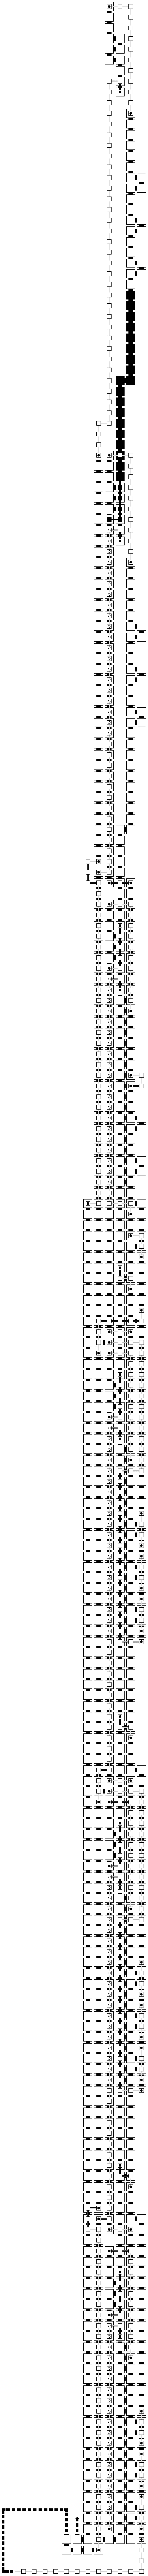
\includegraphics[width=0.45in]{overviews/general/post_warp_3_op}}}%
        ~
        \subcaptionbox{
            Digit 3 - general (seed) overview.
            The black tiles in this figure correspond to the gadget shown in subfigure~\subref{fig:post_warp_2or3_op}.
            \label{fig:post_warp_3_seed_op_overview}
        }{\makebox[0.24\textwidth][c]{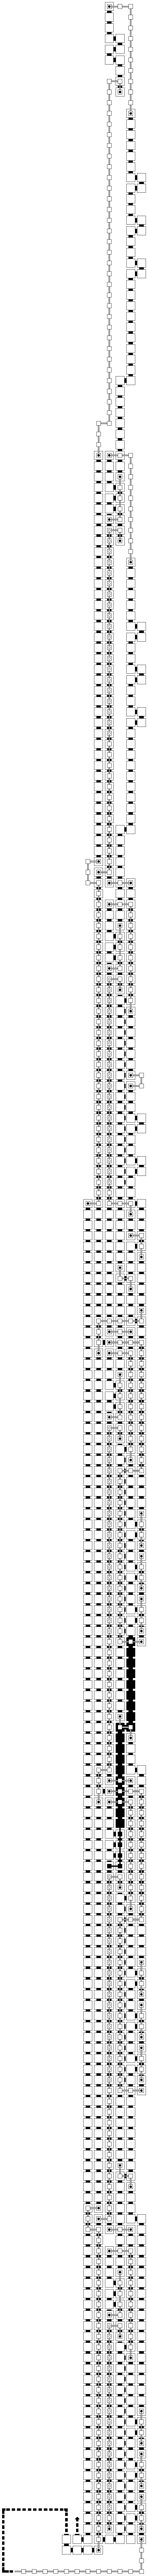
\includegraphics[width=0.45in]{overviews/general/post_warp_3_seed_op}}}%
        ~
        \subcaptionbox{
            Digit 1 - case 1.
            \label{fig:post_warp_1_op_msr_msd}
        }{\makebox[0.24\textwidth][c]{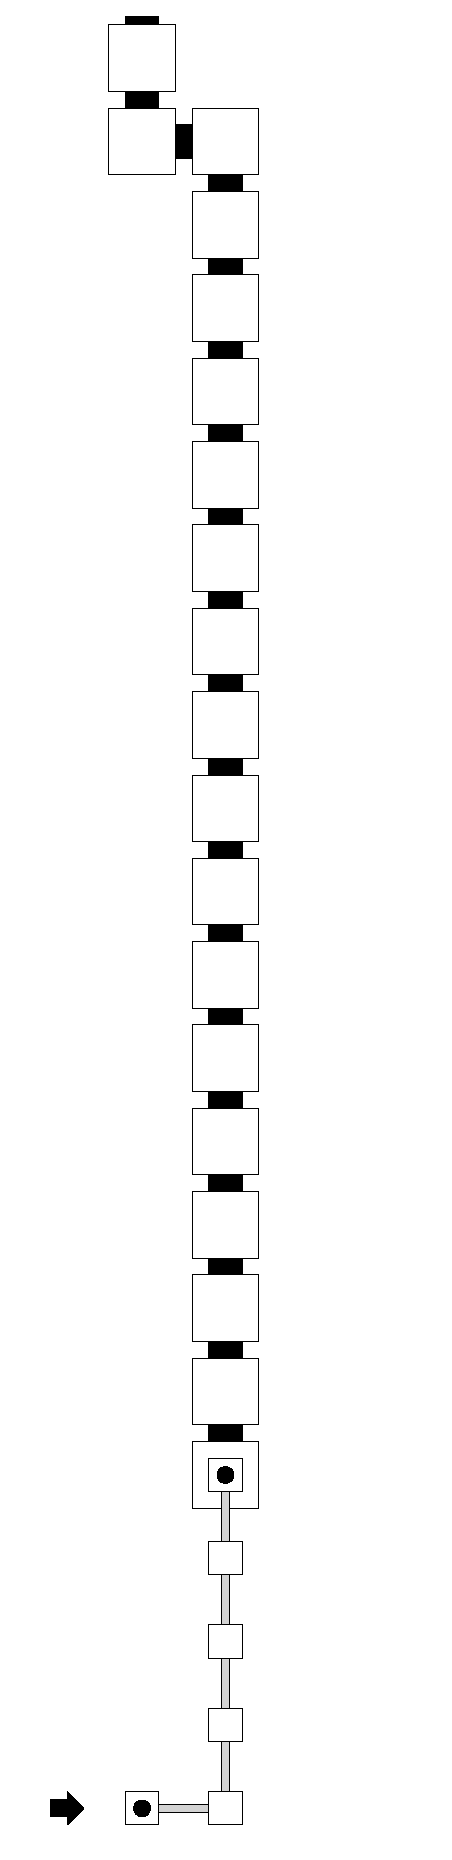
\includegraphics[width=0.45in]{warping_post_warp_case1_digit1_msr}}}%
        ~
    \end{figure}
    \begin{figure}[H]\ContinuedFloat
        \centering
        \subcaptionbox{
            Digit 1 - case 2 overview.
            The black tiles in this figure correspond to the gadget shown in subfigure~\subref{fig:post_warp_1_op_msr_msd}.
            \label{fig:post_warp_1_op_msr_msd_overview}
        }{\makebox[0.24\textwidth][c]{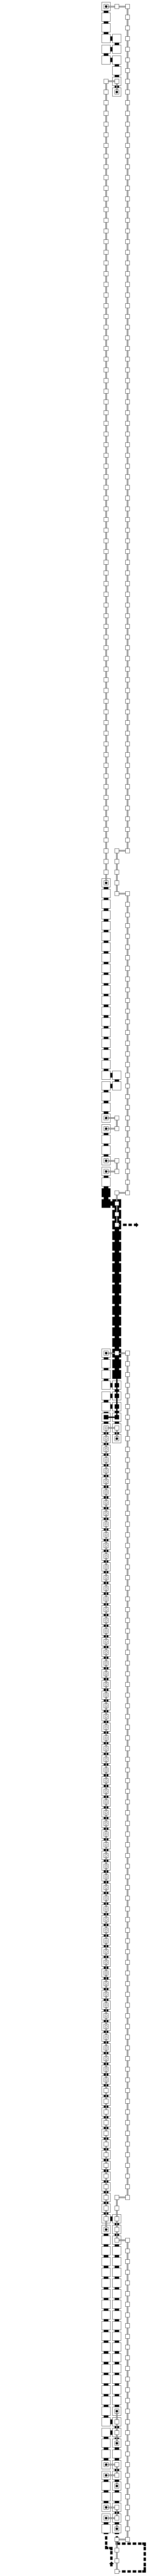
\includegraphics[width=0.45in]{overviews/case1/post_warp_1_op_msr_msd}}}%
        ~
        \subcaptionbox{
            Digit 1 - case 2.
            \label{fig:post_warp_1_op_msr}
        }{\makebox[0.24\textwidth][c]{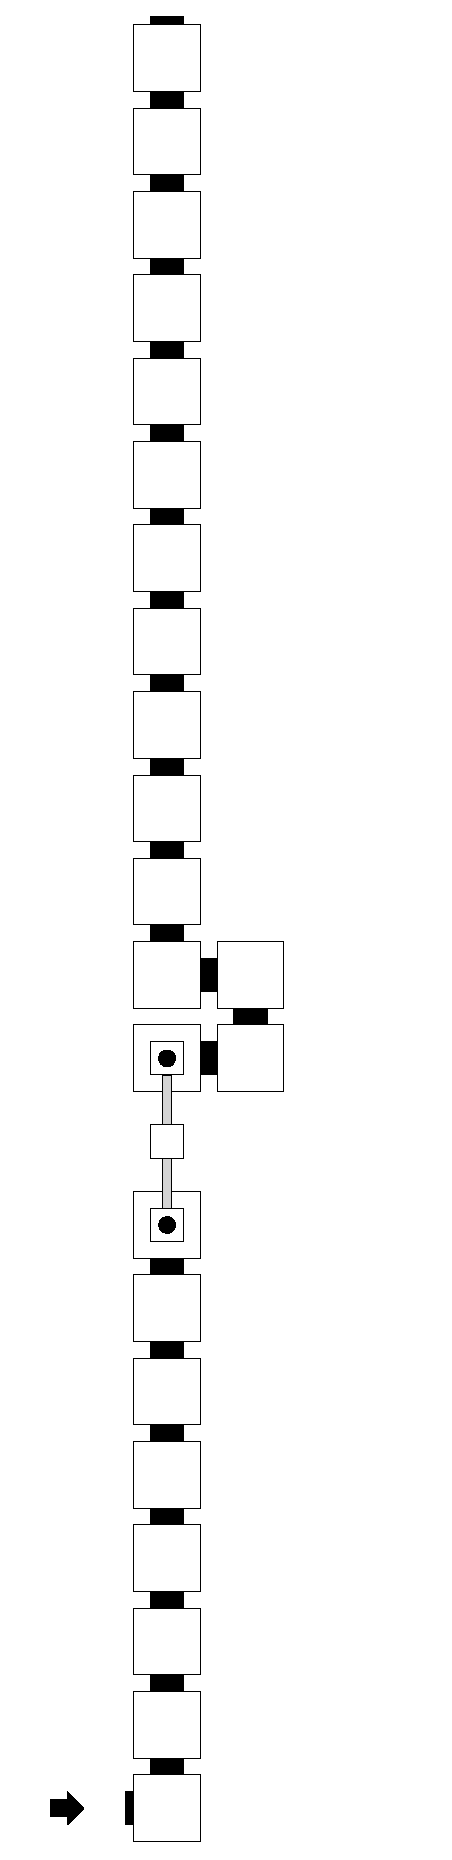
\includegraphics[width=0.45in]{warping_post_warp_case2_digit1_msr}}}%
        ~
        \subcaptionbox{
            Digit 1 - case 2 overview.
            The black tiles in this figure correspond to the gadget shown in subfigure~\subref{fig:post_warp_1_op_msr}.
            \label{fig:post_warp_1_op_msr_overview}
        }{\makebox[0.24\textwidth][c]{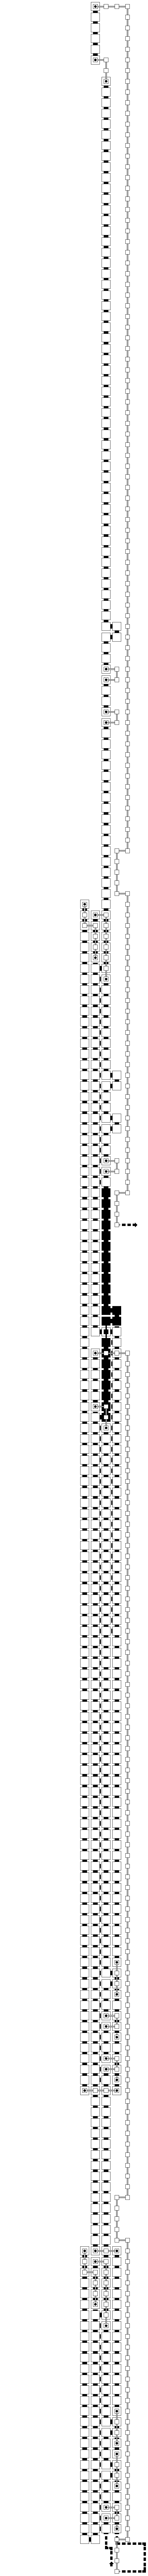
\includegraphics[width=0.45in]{overviews/case2/post_warp_1_op_msr}}}%
        ~
        \subcaptionbox{
            Digit 2 - case 2.
            \label{fig:post_warp_2_op_msr_msd}
        }{\makebox[0.24\textwidth][c]{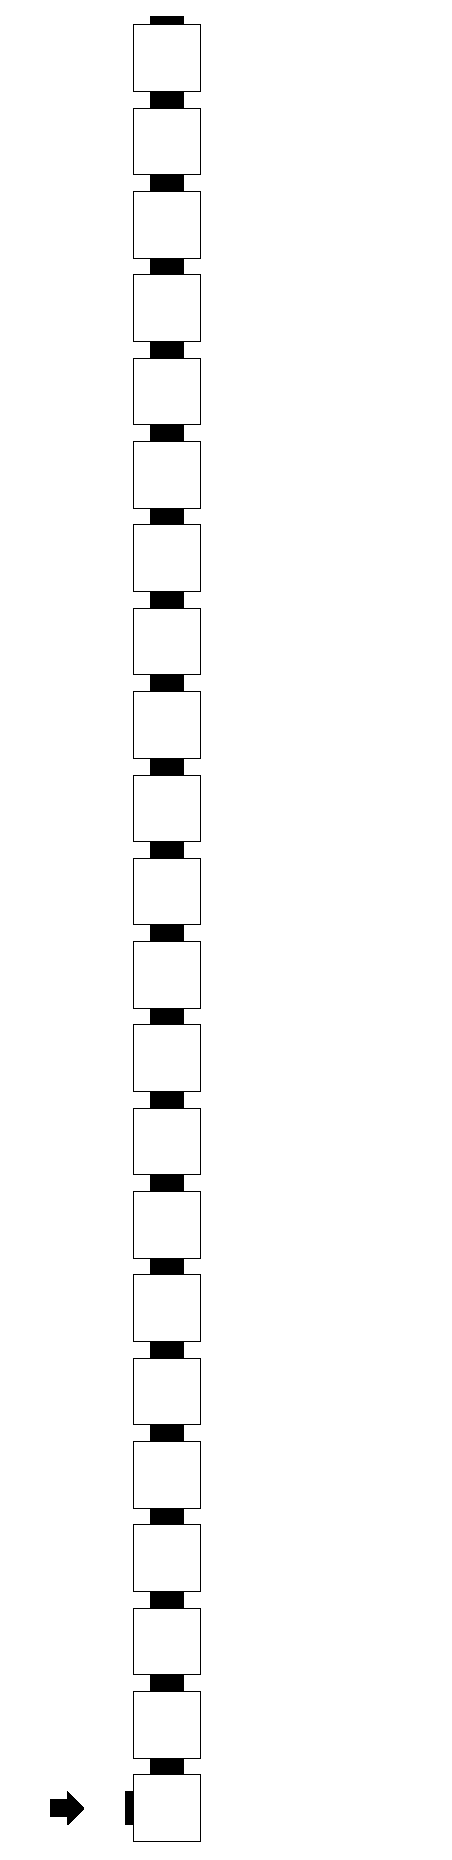
\includegraphics[width=0.45in]{warping_post_warp_case2_digit2_msr}}}%
        ~
    \end{figure}
    \begin{figure}[H]\ContinuedFloat
        \centering
        \subcaptionbox{
            Digit 2 - case 2\\overview.
            The black tiles in this figure correspond to the gadget shown in subfigure~\subref{fig:post_warp_2_op_msr_msd}.
            \label{fig:post_warp_2_op_msr_msd_overview}
        }{\makebox[0.24\textwidth][c]{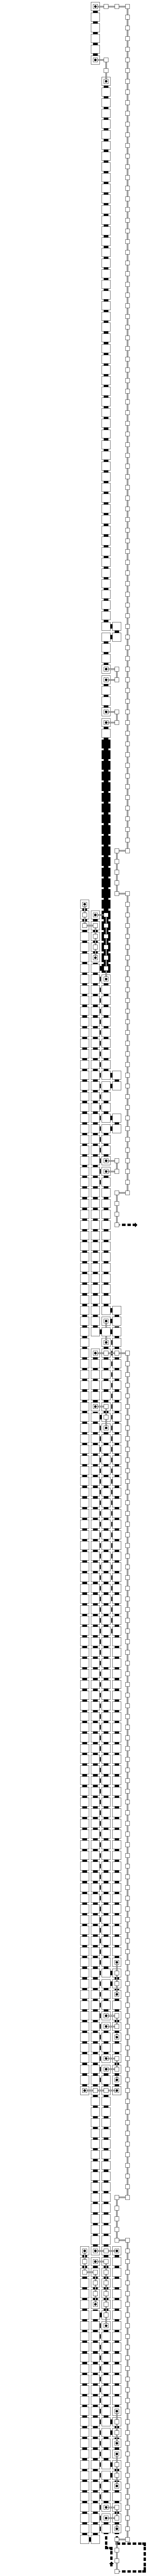
\includegraphics[width=0.45in]{overviews/case2/post_warp_2_op_msr_msd}}}%
        ~
        \subcaptionbox{
            Digit 2 - case 2 (seed) overview.
            The black tiles in this figure correspond to the gadget shown in subfigure~\subref{fig:post_warp_2_op_msr_msd}.
            \label{fig:post_warp_2_seed_op_msr_msd_overview}
        }{\makebox[0.24\textwidth][c]{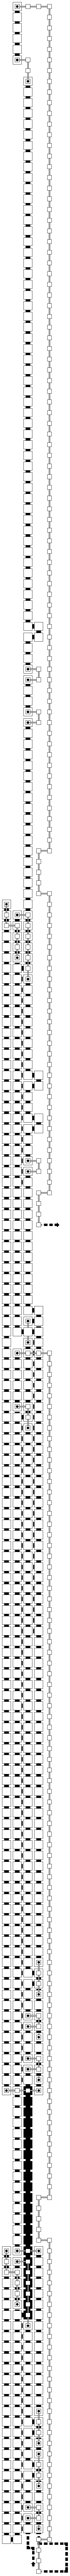
\includegraphics[width=0.45in]{overviews/case2/post_warp_2_seed_op_msr_msd}}}%
        ~
        \subcaptionbox{
            Digit 3 - case 3 overview.
            The black tiles in this figure correspond to the gadget shown in subfigure~\subref{fig:post_warp_2or3_op}.
            \label{fig:post_warp_3_op_msr_msd_overview}
        }{\makebox[0.24\textwidth][c]{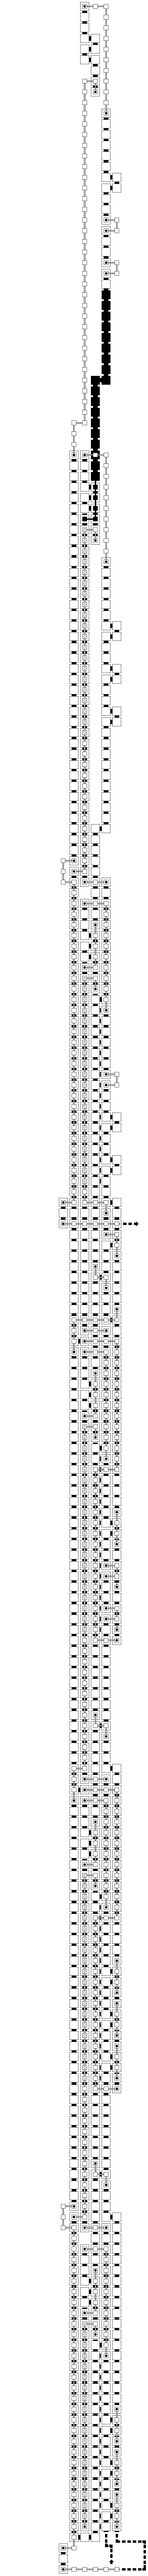
\includegraphics[width=0.45in]{overviews/case3/post_warp_3_op_msr_msd}}}%
        ~
        \subcaptionbox{
            Digit 3 - case 3 (seed) overview.
            The black tiles in this figure correspond to the gadget shown in subfigure~\subref{fig:post_warp_2or3_op}.
            \label{fig:post_warp_3_seed_op_msr_msd_overview}
        }{\makebox[0.24\textwidth][c]{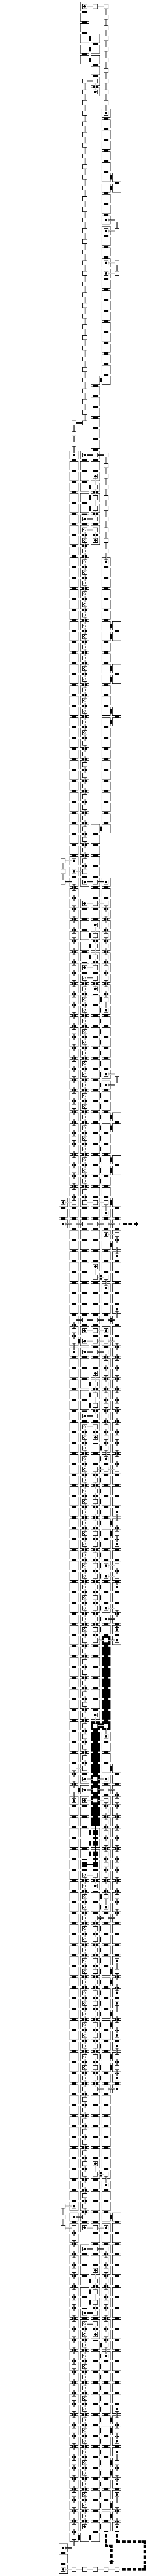
\includegraphics[width=0.45in]{overviews/case3/post_warp_3_seed_op_msr_msd}}}%
        ~
        \caption{\label{fig:post_warp_gadgets} The {\postwarp} gadgets.}
    \end{figure}
\end{itemize}
